\documentclass{article}

\usepackage{color}
\usepackage{url}
\usepackage[utf8]{inputenc}
\usepackage{enumitem}
\usepackage{cmsrb}
\usepackage{graphicx}
\usepackage{lscape}
\usepackage[OT2,T1]{fontenc} 
\usepackage[serbian]{babel}
\usepackage{float}
\usepackage{hvfloat}

\usepackage[unicode]{hyperref}
\hypersetup{colorlinks,citecolor=green,filecolor=green,linkcolor=blue,urlcolor=blue}


\begin{document}

\begin{titlepage}
    \centering

    \newcommand{\HRule}{\rule{\linewidth}{0.5mm}}
    \center
    \textup{\Large Univerzitet u Beogradu\\Matematički fakultet}\\[1.5cm]
    \textup{\Large Projekat iz predmeta Informacioni sistemi 2022/2023.}\\[0.4cm]

    \HRule \\[0.4cm]
    { \huge \bfseries Informacioni sistem srednje škole}\\[0.4cm]
    \HRule \\[1.1cm]
    
    \vspace{6 cm}
	
	\begin{minipage}{0.4\textwidth}
		\begin{flushleft} \large
			\emph{Autori:}\\
			Pavle Savić\\
			Jovan Marković\\
			Mateja Trtica\\
			Lazar Ristić\\		
		\end{flushleft}
	\end{minipage}
	~
	\begin{minipage}{0.5\textwidth}
		\begin{flushright} \large
			\emph{Predmet:}\\ 
			Informacioni sistemi\\
			\emph{Profesor:}\\ 
			Saša Malkov\\
			\emph{Asistent:}\\ 
			Dara Milojković
		\end{flushright}
	\end{minipage}\\[2cm]
	{\large \today}\\[2cm]
\end{titlepage}

\thispagestyle{empty}

\newpage
\renewcommand*\contentsname{Sadržaj:}
\tableofcontents


\newpage
\section{Analiza sistema}

\subsection{Uvod i osnovna ideja}
	Projekat koji je predstavljen u nastavku predstavlja rad u okviru predmeta ``Informacioni sistemi'' na master studijama Matematičkog fakulteta u Beogradu. U njemu su predstavljene neke ideje i znanja stečeni na ovom kursu.
	Osnovna ideja projekta je pravljenje informacionog sistema koji bi mogao da se koristi u nastavi u srednjim školama. Akcenat je stavljen na funkcionalnostima koje pruža nastavnički dnevnik poput evidentiranja časova i upisivanja ocena, ali takođe i pruža pregled relevantnih informacija u zavisnosti od grupe kojoj korisnik pripada. Projekat je predstavljen kao skup raznih dijagrama ( dijagram slučajeva upotrebe, dijagram klasa, dijagram aktivnost, BPMN dijagram i drugi) koji omogućavaju kako specifičniji, tako i opštiji pogled na celokupni sistem, odnosno neke njegove delove.

\subsection{Korisnici sistema}
	U ovom sistemu korisnik može biti prepoznat kao član jedne od pet navedenih grupa korisnika:
\begin{enumerate}
	\item Učenik
	\item Nastavnik
	\item Razredni starešina
	\item Direktor
	\item Administrator
\end{enumerate}
\subsection{Kratak opis}
	Kako se informacije i funkcionalnosti menjaju u zavisnosti od korisnika sistema, tako su u nastavku opisane neke njihove
mogućnosti za rad u ovom sistemu.
	\begin{enumerate}
	\item \textbf{Učenik} \\
	Učenici su najbrojniji korisnici ovog sistema, a ujedno i osnovni razlog njegovog postojanja. Svakom učeniku dodeljeno je odeljenje kojem pripada. Manipulacija podacima im je onemogućena i njihove mogućnosti uglavnom se svode na izdvajanje i pregled njima relevantnih informacija, kao i onemogućen pristup određenim informacijama koje su vezane za druge učenike. Neke od informacija kojima imaju pristup su: 
pregled svojih ocena, rasporeda časova, kalendara aktivnosti, spiska nastavnika i druge. Od omogućenih funkcionalnosti može se izdvojiti prijavljivanje na vannastavne aktivnosti.
 
	\item \textbf{Nastavnik} \\
	Nastavnici predstavljaju predavače u školi. Na početku svake školske godine dodaju im se odeljenje kojima predaju, raspored časova kao i spisak predmeta koje te godine predaju. Ove informacije se mogu izmeniti u toku školske godine. Nastavnici su odgovorni za održavanje nastave i evidentiranje ocena i izostanaka učenika. Što se tiče manipulacije časovima, imaju mogućnost unošenja dopunskog ili dodatnog časa u raspored. Prilikom pregleda ocena učenika sistem nastavnicima omogućava viđenje samo ocena iz svog predmeta.
	\item \textbf{Razredni starešina} \\
	Razredne starešine predstavljaju posebnu grupu nastavnika. Svakom odeljenju je dodat tačno jedan razredni starešina. Razrednim starešinama se dodaju funkcionalnosti za rad sa svojim odeljenjem i njegovim učenicima. Neke od tih funkcionalnosti su opravdavanje izostanaka i izricanje lakše disciplinske mere učenicima. Oni takođe imaju mogućnost pregleda ocena svojih učenika iz svih predmeta.
	\item \textbf{Direktor} \\
	 Direktor je upravni organ svake škole. Njegove nadležnosti tiču se pitanja kao što su aktivnosti u toku godine i pravljenje finansijskih izveštaja. Od funkcionalnosti takođe imaju i pravljenje izmena u dnevniku i izricanja težih disciplinskih mera učenicima. Odgovoran je za blagovremeno rešavanje raznih problema koji nastaju u toku školske godine. Direktor ima pristup informacijama o svim nastavnicima, učenicima, njihovim ocenama, kao i informacijama o odeljenjima.
	\item \textbf{Administrator} \\ 
	Administratori su odgovorni za funkcionisanje sistema. Imaju pristup velikoj količini podataka, kao i razne funkcionalnosti koje se tiču registrovanju korisnika u sistem, kao i deaktivaciju njihovih naloga. Oni takođe mogu ažurirati informacije o korisnicima. Odgovorni su za uspostavljanje uslova za početak nove školske godine, a to je omogućeno kroz kreiranje kalendara aktivnosti, rasporeda časova, novih odeljenja i dnevnika ocena, kao i kroz modifikaciju postojećih.
\end{enumerate}

\newpage
\section{Dijagrami toka podataka}

\begin{figure} [!ht]
    \begin{center}
        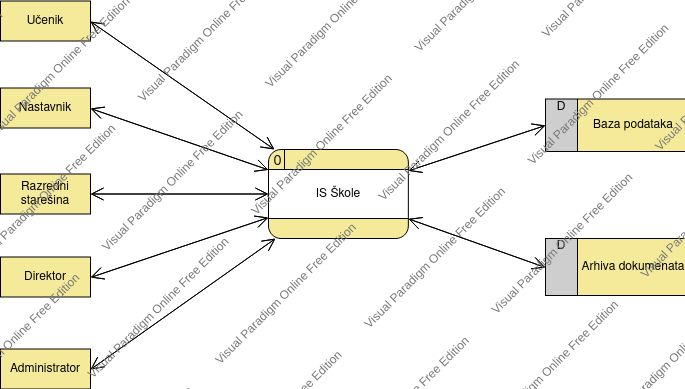
\includegraphics[scale=0.5]{imgs/dijagram_konteksta.png}
    \end{center}
\caption{Dijagram konteksta sistema}
\end{figure}

\begin{figure} [!ht]
    \begin{center}
        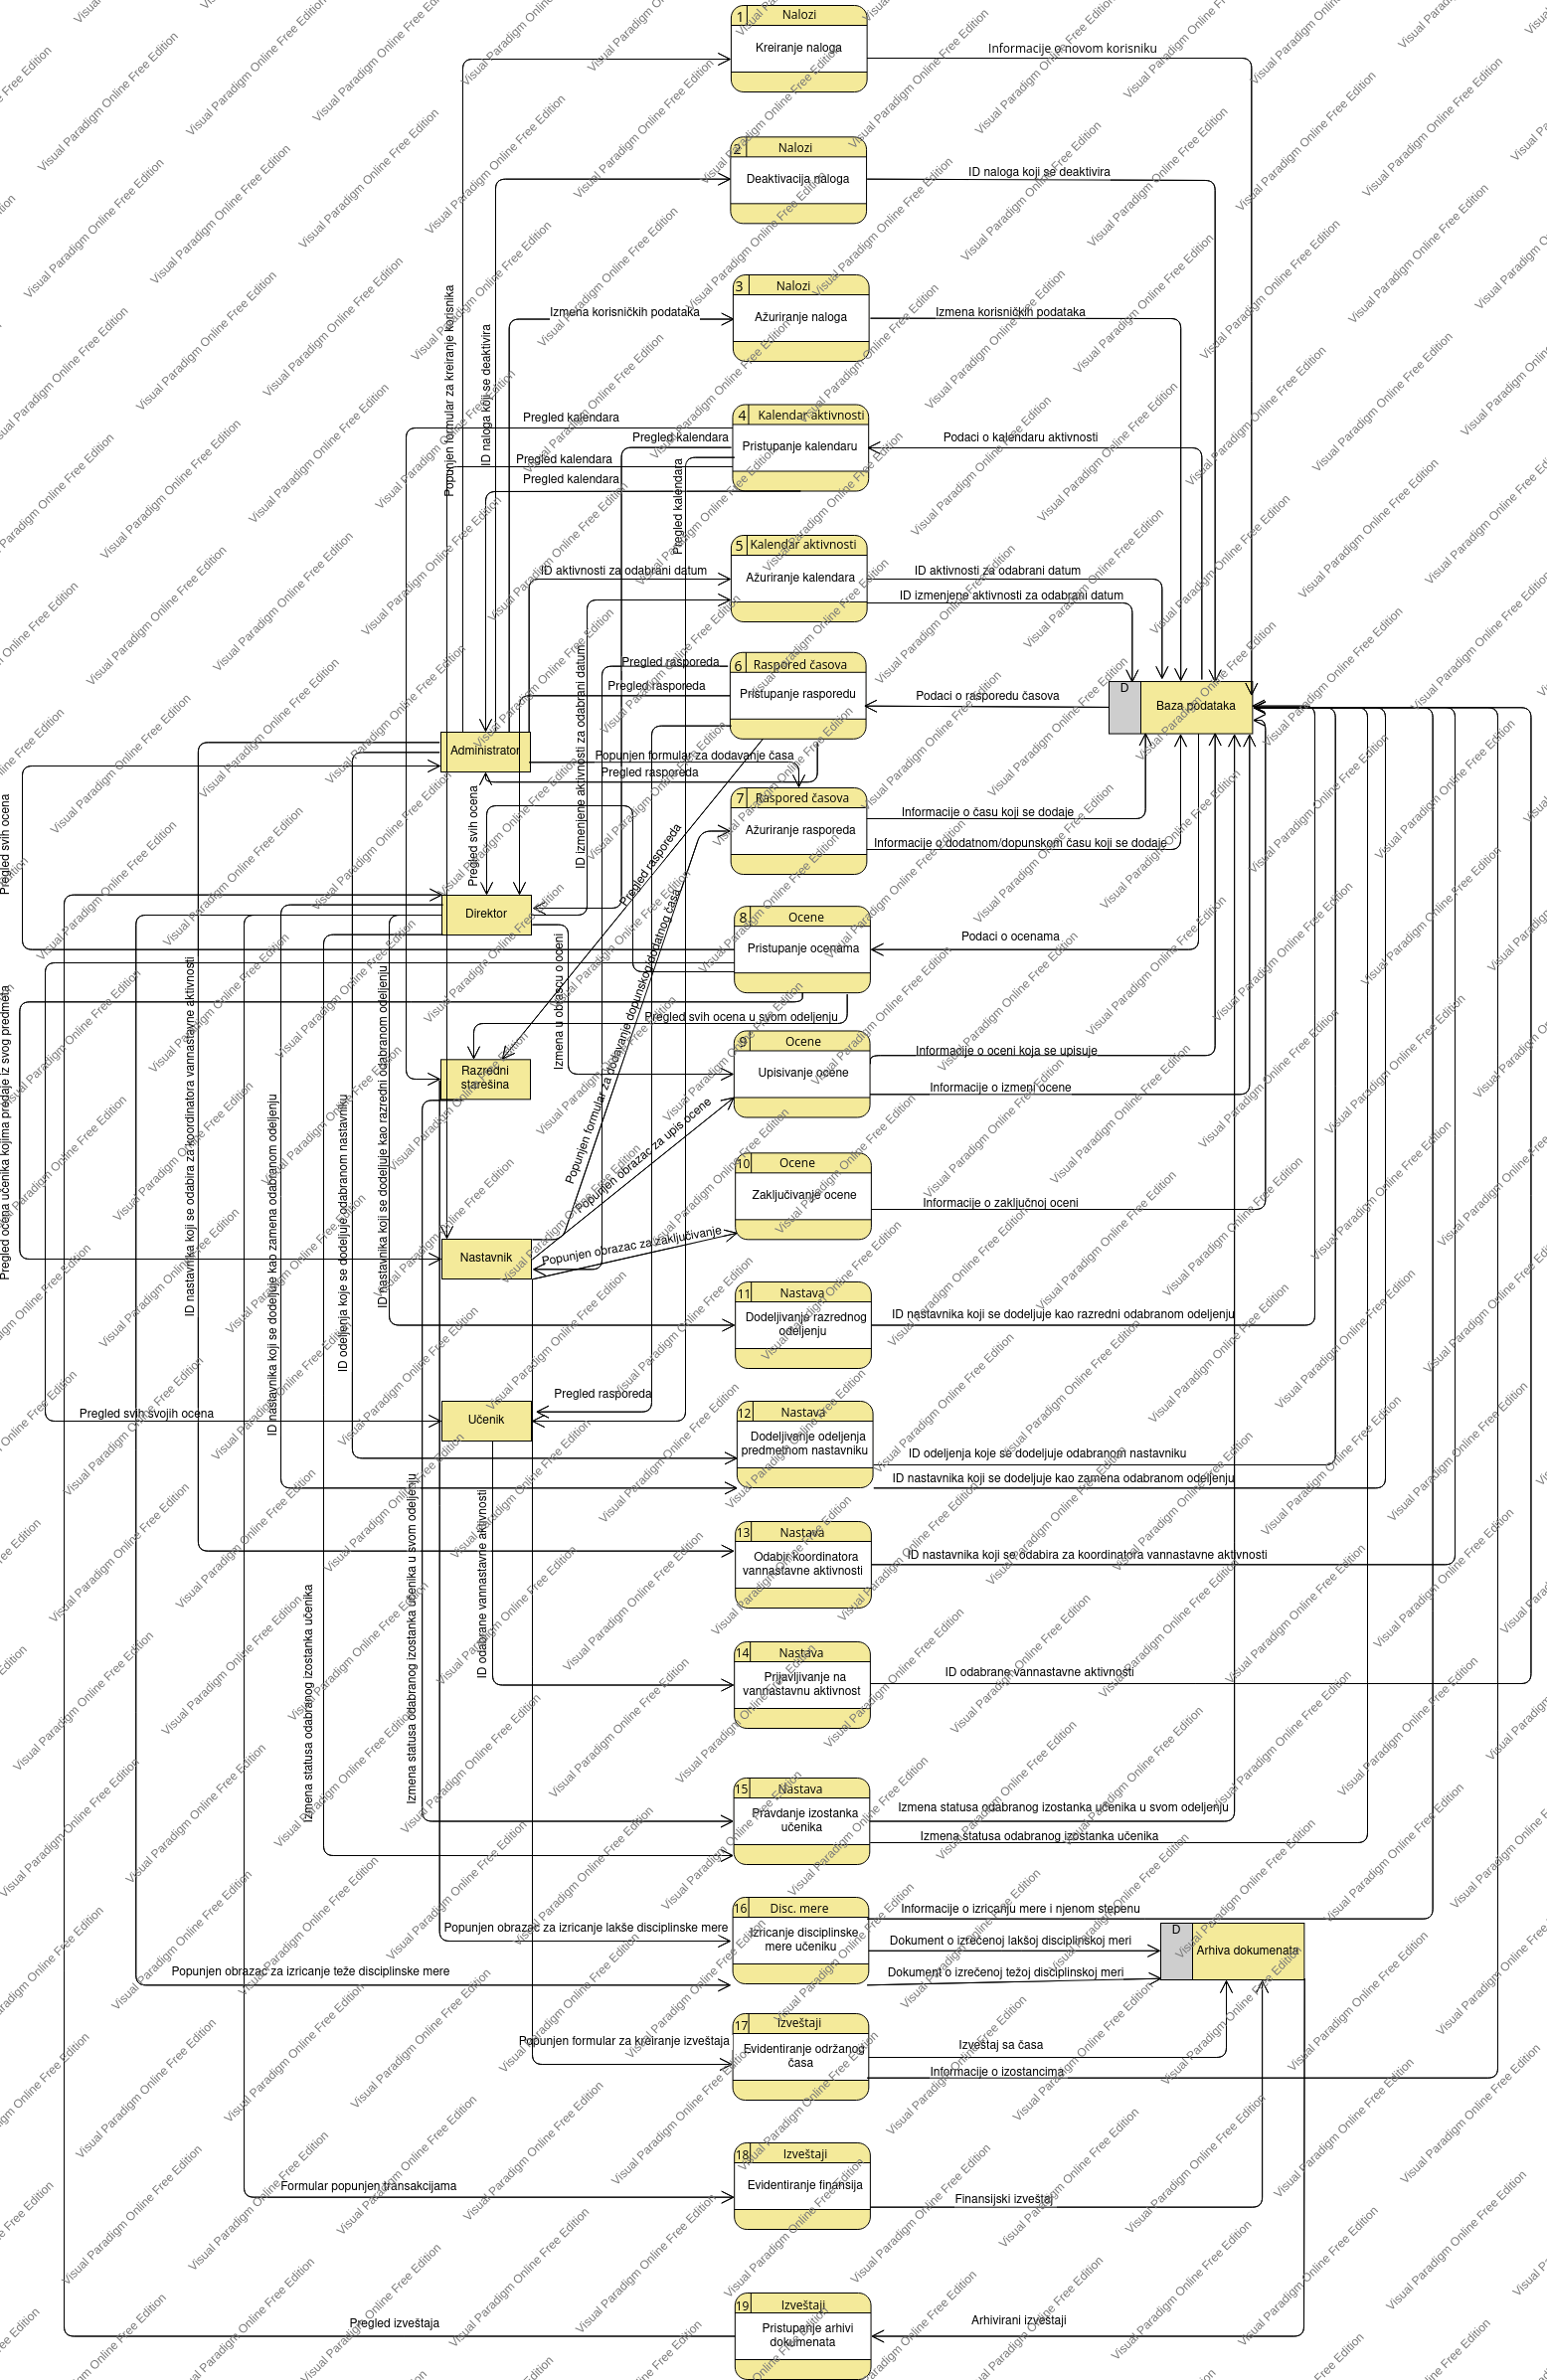
\includegraphics[scale=0.2]{imgs/dijagram_nivoa_0.png}
    \end{center}
\caption{Dijagram toka podataka nivoa 0}
\end{figure}

\newpage
\section{Slučajevi upotrebe}

\subsection{Aktivnosti Učenika}

\begin{figure} [!ht]
    \begin{center}
        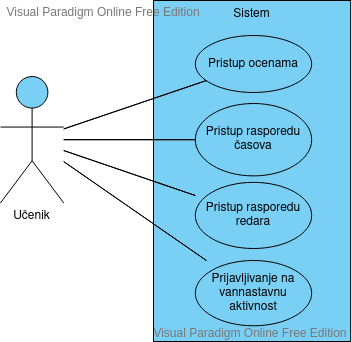
\includegraphics[scale=0.6]{imgs/ucenik_use_case.png}
    \end{center}
\caption{Dijagram slučajeva upotrebe Učenika}
\end{figure}


\subsubsection{Slučaj upotrebe: Učenik pristupa svojim ocenama} 
1. \textbf{Kratak opis:} Učenik pristupa svojim ocenama iz željenog predmeta. Učenik filtrira ocene po željenom kriterijumu. \\

2. \textbf{Učesnici:}
\begin{enumerate} [label=(\alph*)]
\item Učenik
\end{enumerate} 

3. \textbf{Preduslov:} Učenik je registrovani korisnik sistema. Učenik ima pristup Internetu. Sistem je u funkciji. Učenik je upisan na predmet. \\

4. \textbf{Postuslov:} Učenik je pristupio elektronskom dnevniku i pročitao potrebne informacije o ocenama.\\

5. \textbf{Osnovni tok:} 
\begin{enumerate} [label=(\alph*)]
\item Učenik pristupa stranici sa listom predmeta koje pohađa
\item Učenik pritiska dugme za pristup ocenama iz željenog predmeta
\item Sistem prikazuje sve ocene učenika iz tog predmeta u tekućoj školskoj godini
\item Učenik pritiska na dugme za filtriranje ocena
\item Sistem prikazuje učeniku polja za filtriranje
\item Učenik unosi željeni kriterijum filtriranja
\item Sistem filtrira ocene
\item Sistem prikazuje ocene filtrirane po željenom kriterijumu
\end{enumerate}

6. \textbf{Alternativni tokovi:}
\begin{enumerate} [label=(\roman*)]
\item Učenik nema ocene za prikaz - Ako u koraku (b) učenik želi da pristupi ocenama iz predmeta iz kojeg nije upisana nijedna ocena sistem ga obaveštava odgovarajućom porukom. Proces se nastavlja iz koraka (a).
\item Nijedna ocena ne ispunjava kriterijum - Ako u koraku (g) sistem utvrdi da nijedna ocena ne ispunjava željeni kriterijum obaveštava učenika odgovarajućom porukom. Proces se nastavlja iz koraka (c).
\end{enumerate}

7. \textbf{Podtokovi}: - \\

8. \textbf{Specijalni zahtevi}: - \\

9. \textbf{Dodatne informacije}: Klikom na proizvoljnu ocenu učenik može videti tip ocene (kontrolni/pismeni/usmeni/aktivnost) i napomenu (ako je uneta). Kriterijum filtriranja su tip ocene i polugodište (prvo ili drugo). \\


\begin{figure} [!ht]
    \begin{center}
        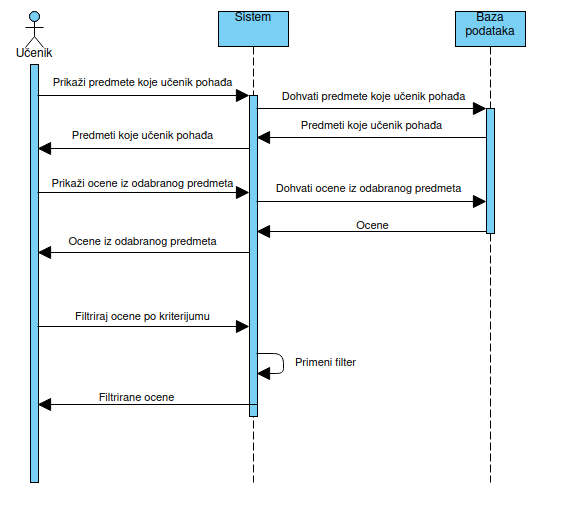
\includegraphics[scale=0.5]{imgs/Dijagram_sekvence_ucenik_pristupa_ocenama.png}
    \end{center}
\caption{Dijagram sekvence Pristupanje ocenama}
\end{figure}


\newpage
\subsubsection{Slučaj upotrebe: Učenik pristupa rasporedu časova} 
1. \textbf{Kratak opis:} Učenik pristupa rasporedu časova odeljenja kom pripada u željenoj smeni. \\

2. \textbf{Učesnici:}
\begin{enumerate} [label=(\alph*)]
\item Učenik
\end{enumerate} 

3. \textbf{Preduslov:} Učenik je registrovani korisnik sistema. Učenik ima pristup Internetu. Sistem je u funkciji. Učenik je dodeljen odeljenju. \\

4. \textbf{Postuslov:} Učenik je pristupio rasporedu časova i pročitao potrebne informacije. \\

5. \textbf{Osnovni tok:} 
\begin{enumerate} [label=(\alph*)]
\item Učenik pristupa početnoj stranici rasporeda časova
\item Sistem prikazuje učeniku padajući meni za izbor odeljenja i smene
\item Učenik pritiskom na željene opcije bira odeljenje i smenu
\item Učenik pritiskom na dugme potvrđuje unos 
\item Sistem obrađuje zahtev
\item Sistem prikazuje učeniku raspored časova njegovog odeljenja u željenoj smeni 
\end{enumerate}

6. \textbf{Alternativni tokovi:}
\begin{enumerate} [label=(\roman*)]
\item Raspored časova ne postoji - Ako u koraku (e) sistem utvrdi da odeljenju nije dodeljen raspored časova (za odabranu smenu) obaveštava učenika odgovarajućom porukom. Proces se nastavlja iz koraka (b).

\end{enumerate}

7. \textbf{Podtokovi}: - \\

8. \textbf{Specijalni zahtevi}: - \\

9. \textbf{Dodatne informacije}: Prema pravilniku škole za svako odeljenje prepodnevna i poslepodnevna smena smenjuju se na nedeljnom nivou. \\

\begin{figure} [!ht]
    \begin{center}
        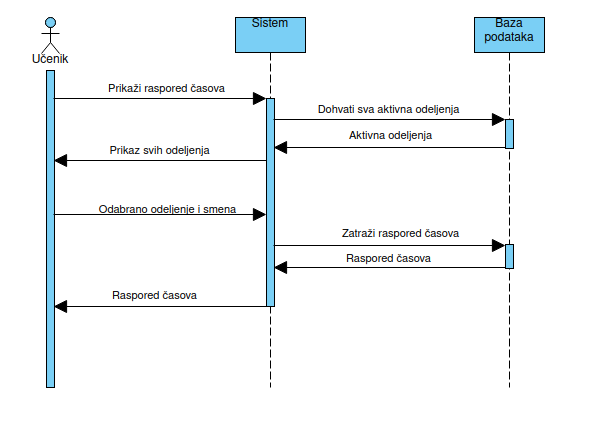
\includegraphics[scale=0.5]{imgs/Dijagram_sekvence_ucenik_pristupa_rasporedu.png}
    \end{center}
\caption{Dijagram sekvence Pristupanje rasporedu časova}
\end{figure}

\newpage
\subsubsection{Slučaj upotrebe: Učenik pristupa kalendaru aktivnosti} 
1. \textbf{Kratak opis:} Učenik pristupa kalendaru aktivnosti odabranog meseca. \\ 

2. \textbf{Učesnici:}
\begin{enumerate} [label=(\alph*)]
\item Učenik
\end{enumerate} 

3. \textbf{Preduslov:} Učenik je registrovani korisnik sistema. Učenik ima pristup Internetu. Sistem je u funkciji. \\

4. \textbf{Postuslov:} Učenik je pristupio kalendaru aktivnosti i pročitao potrebne informacije. \\

5. \textbf{Osnovni tok:} 
\begin{enumerate} [label=(\alph*)]
\item Učenik pristupa početnoj stranici kalendara aktivnosti
\item Sistem prikazuje učeniku padajući meni za izbor godine i meseca
\item Učenik pritiskom na željene opcije bira godinu i mesec
\item Učenik pritiskom na dugme potvrđuje unos 
\item Sistem obrađuje zahtev
\item Sistem prikazuje kalendar aktivnosti za odabrani mesec i godinu
\end{enumerate}


6. \textbf{Alternativni tokovi:}
\begin{enumerate} [label=(\roman*)]
\item Kalendar aktivnosti ne postoji - Ako u koraku (e) sistem utvrdi kalendar aktivnosti za odabrani mesec i godinu nije kreiran obaveštava učenika odgovarajućom porukom. Proces se nastavlja iz koraka (b).
\end{enumerate}

7. \textbf{Podtokovi}: - \\

8. \textbf{Specijalni zahtevi}: - \\

9. \textbf{Dodatne informacije}: Pre početku školske godine administrator kreira kalendar aktivnosti za nastupajuću školsku godinu. \\

\begin{figure} [!ht]
    \begin{center}
        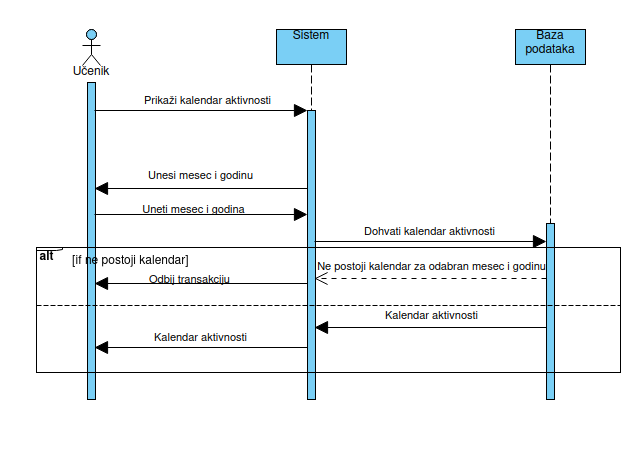
\includegraphics[scale=0.5]{imgs/Dijagram_sekvence_ucenik_pristupa_kalendaru.png}
    \end{center}
\caption{Dijagram sekvence Pristupanje kalendaru aktivnosti}
\end{figure}

\newpage
\subsubsection{Slučaj upotrebe: Učenik se prijavljuje na vannastavnu aktivnost} 
1. \textbf{Kratak opis:} Učenik odabira željenu vannastavnu aktivnost. Sistem proverava raspoloživost, čuva prijavu i o tome obaveštava učenika. \\

2. \textbf{Učesnici:}
\begin{enumerate} [label=(\alph*)]
\item Učenik
\end{enumerate} 

3. \textbf{Preduslov:} Učenik je registrovani korisnik sistema. Učenik ima pristup Internetu. Sistem je u funkciji. Za željenu aktivnost odabran je koordinator (neko od nastavnika). \\

4. \textbf{Postuslov:} Sistem je evidentirao prijavu učenika na vannastavnu aktivnost. Baza je ažurirana. \\

5. \textbf{Osnovni tok:} 
\begin{enumerate} [label=(\alph*)]
\item Učenik pristupa stranici sa listom vannastavnih aktivnosti
\item Učenik pritiska na željenu aktivnost
\item Sistem prikazuje kratak opis odabrane aktivnosti
\item Učenik pritiska dugme za prijavu na željenu aktivnost
\item Sistem prikazuje dialog box (da/ne) i pita učenika da li želi da se prijavi
\item Učenik potvrđuje prijavu
\item Sistem vrši proveru raspoloživosti odabrane aktivnosti
\item Sistem čuva prijavu
\item Sistem obaveštava učenika o uspešnoj prijavi na vannastavnu aktivnost
\end{enumerate}

6. \textbf{Alternativni tokovi:}
\begin{enumerate} [label=(\roman*)]
\item Učenik ne potvrđuje prijavu - Ako u koraku (f) učenik odgovori odrično ili ugasi dialog box sistem ne evidentira prijavu. Proces se nastavlja iz koraka (c). 
\item Sva mesta na izabranoj aktivnosti popunjena - Ako u koraku (g) sistem utvrdi da učenik pokušava da se prijavi na aktivnost na kojoj su sva mesta popunjena, sistem o tome obaveštava učenika i odbija prijavu. Proces se nastavlja iz koraka (a).
\item Učenik se prijavljuje na već prijavljenu aktivnost - Ako u koraku (g) sistem utvrdi da učenik pokušava ponovno da se prijavi na aktivnost na koju je već prijavljen, sistem o tome obaveštava učenika i odbija prijavu. Proces se nastavlja iz koraka (a).

\end{enumerate}

7. \textbf{Podtokovi}: - \\

8. \textbf{Specijalni zahtevi}: - \\

9. \textbf{Dodatne informacije}: Škola nudi vannastavne aktivnosti kao što su: sportske sekcije, glumačka sekcija, muzička sekcija, besedništvo. Broj raspoloživih mesta specifičan je za svaku sekciju. Obaveze učenika koji su prijavljeni na neku vannastavnu aktivnost uzimaju se u obzir kao kriterijum prilikom pravljenja rasporeda časova. \\

\begin{figure} [!ht]
    \begin{center}
        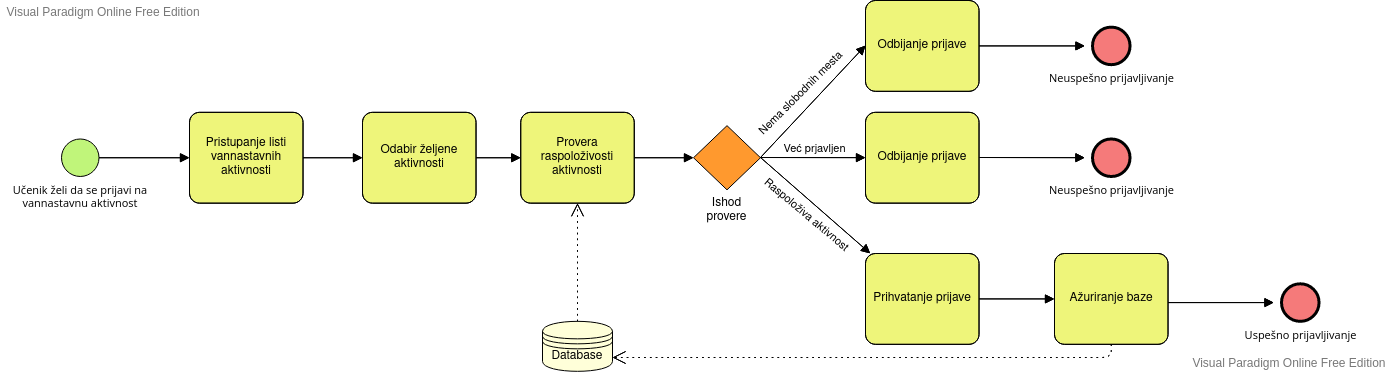
\includegraphics[scale=0.34]{imgs/BPMN_prijava_na_aktivnost.png}
    \end{center}
\caption{BPMN dijagram procesa Prijavljivanje na vannastavnu aktivnost}
\end{figure}


\newpage
\subsection{Aktivnosti Nastavnika}

\begin{figure} [!ht]
    \begin{center}
        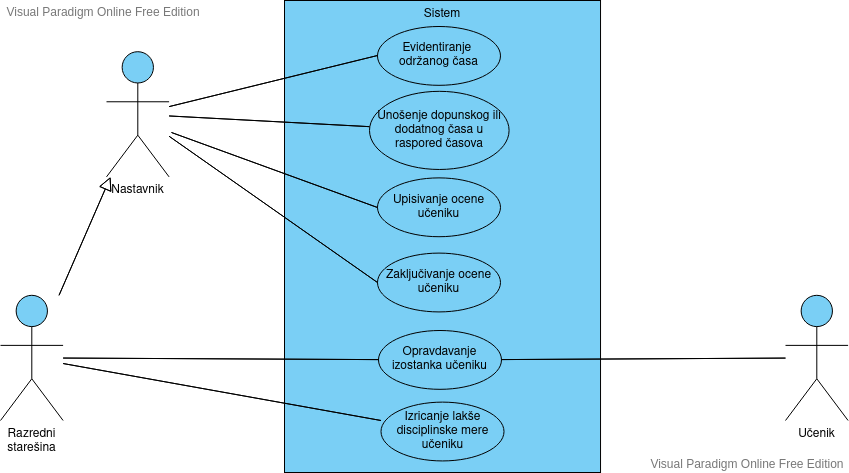
\includegraphics[scale=0.45]{imgs/nastavnik_use_case.png}
    \end{center}
\caption{Dijagram slučajeva upotrebe Nastavnika i Razrednog starešine kao njegove specijalizacije}
\end{figure}

\newpage
\subsubsection{Slučaj upotrebe: Nastavnik evidentira održani čas} 
1. \textbf{Kratak opis:} Nakon održanog časa nastavnik unosi informacije o nastavnoj temi pređenoj na tom času i upisuje odsutne učenike. Sistem validira i čuva unete podatke i obaveštava nastavnika o uspešno unetom izveštaju.\\

2. \textbf{Učesnici:}
\begin{enumerate} [label=(\alph*)]
\item Nastavnik
\end{enumerate} 

3. \textbf{Preduslov:} Nastavnik je registrovani korisnik sistema. Nastavnik ima pristup Internetu. Sistem je u funkciji. \\

4. \textbf{Postuslov:} Izveštaj sa održanog časa je unet u arhivu dokumenata sistema. Odsutnim učenicima zabeležen je izostanak. Baza je ažurirana. \\

5. \textbf{Osnovni tok:} 
\begin{enumerate} [label=(\alph*)]
\item Nastavnik pristupa listi održanih časova
\item Nastavnik pritiska dugme za kreiranje novog izveštaja sa časa
\item Sistem prikazuje formular za kreiranje novog izveštaja sa časa
\item Nastavnik unosi tražene podatke 
\item Nastavnik pritiskom na dugme potvrđuje unos
\item Sistem vrši validaciju podataka
\item Sistem čuva podatke
\item Sistem vraća poruku o uspešno kreiranom izveštaju
\end{enumerate}

6. \textbf{Alternativni tokovi:}
\begin{enumerate} [label=(\roman*)]
\item Nastavnik unosi nevalidne podatke u formular - Ako u koraku (f) sistem utvrdi neispravno polje formulara (prazno obavezno polje, nastavnik ne predaje odabranom odeljenju) sistem obaveštava nastavnika obeležavanjem nevalidnog polja. Nastavnik ispravlja neispravno polje. Proces se nastavlja iz koraka (d).
\end{enumerate}

7. \textbf{Podtokovi}: - \\

8. \textbf{Specijalni zahtevi}: - \\

9. \textbf{Dodatne informacije}: Obavezna polja formulara jesu: datum, odeljenje, nastavna tema i spisak odsutnih učenika. Opciona polja su: literatura za temu, domaći zadatak i napomene. \\

\begin{figure} [!ht]
    \begin{center}
        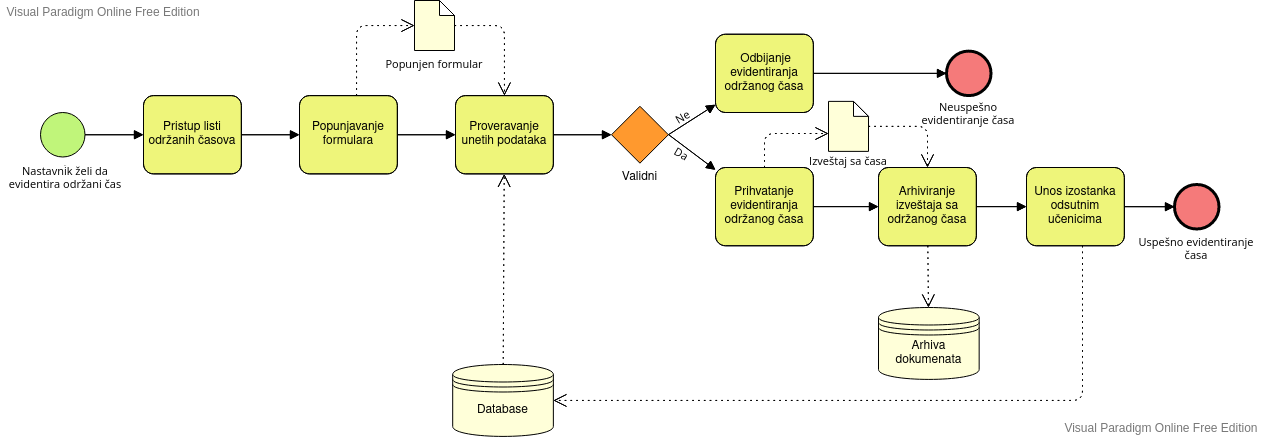
\includegraphics[scale=0.36]{imgs/BPMN_evidentiranje_casa.png}
    \end{center}
\caption{BPMN dijagram procesa Evidentiranje održanog časa}
\end{figure}


\subsubsection{Slučaj upotrebe: Nastavnik unosi dopunski ili dodatni čas u raspored časova} 
1. \textbf{Kratak opis:} U dogovoru sa zainteresovanim učenicima nastavnik dodaje dopunski ili dodatni čas u postojeći raspored časova. Sistem validira i čuva unete izmene i obaveštava nastavnika o uspešno ažuriranom rasporedu. \\

2. \textbf{Učesnici:}
\begin{enumerate} [label=(\alph*)]
\item Nastavnik
\end{enumerate} 

3. \textbf{Preduslov:} Nastavnik je registrovani korisnik sistema. Nastavnik ima pristup Internetu. Sistem je u funkciji. Raspored časova je kreiran. \\

4. \textbf{Postuslov:} Dopunski ili dodatni čas dodat je u raspored časova. Baza je ažurirana. \\

5. \textbf{Osnovni tok:} 
\begin{enumerate} [label=(\alph*)]
\item Nastavnik pristupa stranici na kojoj je prikazan raspored časova
\item Nastavnik pritiska na odabrani dana  
\item Sistem otvara formular za upis podataka o času koji se dodaje u raspored
\item Nastavnik popunjava formular traženim podacima
\item Nastavnik pritiskom na dugme potvrđuje slanje zahteva za unos časa u raspored
\item Sistem validira unete podatke
\item Sistem vrši proveru da li je došlo do preklapanja u rasporedu časova
\item Sistem čuva podatke
\item Sistem vraća poruku o uspešno ažuriranom rasporedu
\end{enumerate}

6. \textbf{Alternativni tokovi:}
\begin{enumerate} [label=(\roman*)]
\item Nastavnik unosi nevalidne podatke u formular - Ako u koraku (f) sistem utvrdi nevalidne podatke (obavezna polja ostala nepopunjena) obaveštava nastavnika obeležavanjem neispravnog polja. Nastavnik ispravlja neispravno polje. Proces se nastavlja iz koraka (d).
\item Neuspešna izmena rasporeda - Ako u koraku (g) sistem utvrdi preklapanje u rasporedu časova obaveštava nastavnika ispisivanjem časa koji se u rasporedu već nalazi u tom terminu. Nastavnik bira drugi dan i proces se nastavlja iz koraka (b).

\end{enumerate}

7. \textbf{Podtokovi}: - \\

8. \textbf{Specijalni zahtevi}: Nastavnik dodatnu/dopunsku nastavu može zakazati samo u terminu 7. časa u prvoj smeni (predčas u drugoj smeni). \\

9. \textbf{Dodatne informacije}: Obavezna polja formulara su: naziv predmeta, odeljenje, broj kabineta, tip časa (dopunska/dodatna). Opciono polje je napomena. \\

\begin{figure} [!ht]
    \begin{center}
        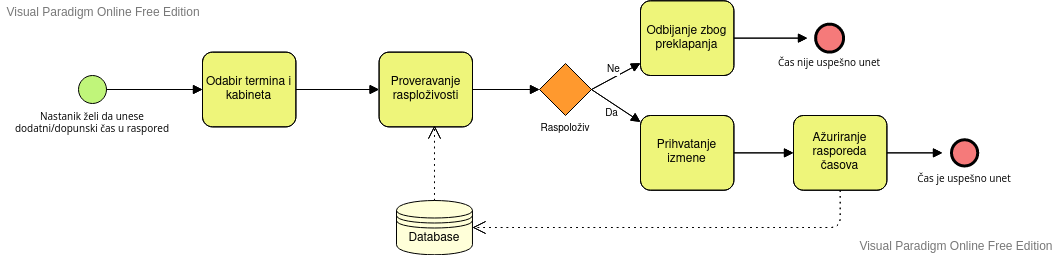
\includegraphics[scale=0.4]{imgs/BPMN_zakazivanje_dopunske_dodatne.png}
    \end{center}
\caption{BPMN dijagram procesa Unošenje dopunskog/dodatnog časa u raspored}
\end{figure}


\begin{figure} [!ht]
    \begin{center}
        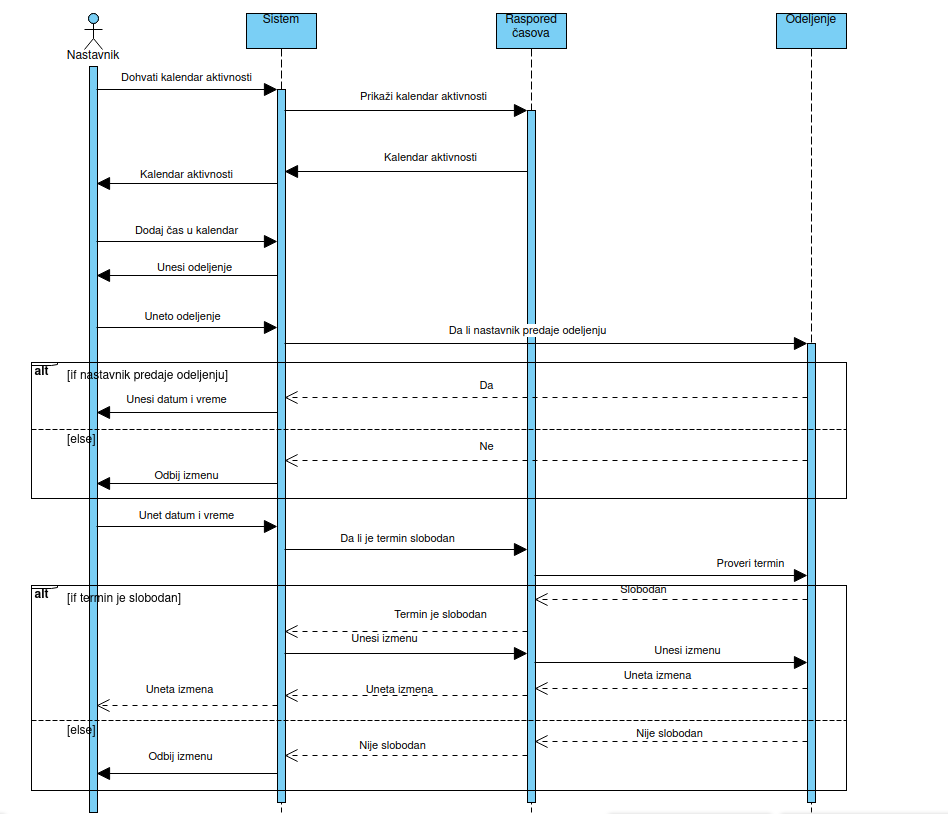
\includegraphics[scale=0.4]{imgs/Dijagram_sekvence_nastavnik_dodaje_cas.png}
    \end{center}
\caption{Dijagram sekvence Unošenje dopunskog/dodatnog časa u raspored}
\end{figure}


\newpage
\subsubsection{Slučaj upotrebe: Nastavnik upisuje ocenu učeniku} 
1. \textbf{Kratak opis:} Nakon održane provere znanja (pismene ili usmene) nastavnik unosi ostvarenu ocenu učenika u elektronski dnevnik. Sistem validira i čuva unetu ocenu i obaveštava nastavnika o uspešno unetoj oceni.  \\

2. \textbf{Učesnici:}
\begin{enumerate} [label=(\alph*)]
\item Nastavnik
\end{enumerate} 

3. \textbf{Preduslov:} Nastavnik je registrovani korisnik sistema. Nastavnik ima pristup Internetu. Sistem je u funkciji. \\

4. \textbf{Postuslov:} Ocena učenika uneta je u elektronski dnevnik. Baza je ažurirana.\\

5. \textbf{Osnovni tok:} 
\begin{enumerate} [label=(\alph*)]
\item Nastavnik pristupa listi učenika podeljenih po odeljenjima kojima predaje
\item Nastavnik vrši pretragu i pritiska dugme za pristup ocenama kod odgovarajućeg učenika
\item Sistem otvara stranicu sa ocenama odgovarajućeg učenika
\item Nastavnik pritiska na dugme za unos nove ocene
\item Sistem prikazuje obrazac za unos nove ocene
\item Nastavnik popunjava obrazac
\item Nastavnik pritiskom na dugme potvrđuje unos ocene
\item Sistem validira unete podatke
\item Sistem čuva unetu ocenu
\item Sistem vraća poruku o uspešno unetoj oceni
\end{enumerate}

6. \textbf{Alternativni tokovi:}
\begin{enumerate} [label=(\roman*)]
\item Nastavnik unosi nevalidne podatke u obrazac - Ako u koraku (h) sistem utvrdi nevalidnu ocenu (ocena nije od 1 do 5) ili prazno obavezno polje obaveštava nastavnika obeležavanjem neispravnog polja. Nastavnik ispravlja neispravno polje. Proces se nastavlja iz koraka (f).
\end{enumerate}

7. \textbf{Podtokovi}: - \\

8. \textbf{Specijalni zahtevi}: - \\

9. \textbf{Dodatne informacije}: Obavezna polja obrasca su: ocena i tip ocene (kontrolni/pismeni/usmeni/aktivnost). Opciono polje je napomena. \\

\begin{figure} [!ht]
    \begin{center}
        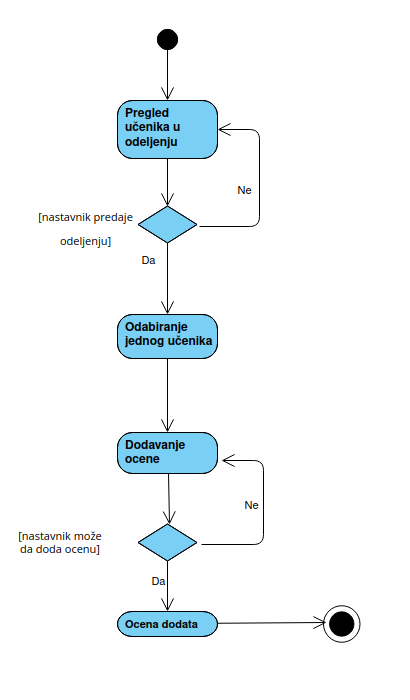
\includegraphics[scale=0.4]{imgs/Dijagram_aktivnosti_nastavnik_upisuje_ocenu.png}
    \end{center}
\caption{Dijagram aktivnosti Upisivanje ocene učeniku}
\end{figure}

\newpage
\subsubsection{Slučaj upotrebe: Nastavnik zaključuje ocenu učeniku} 
1. \textbf{Kratak opis:} Na osnovu ostvarenih ocena u toku školske godine nastavnik unosi zaključnu ocenu učenika u elektronski dnevnik. Sistem validira i čuva unetu ocenu i obaveštava nastavnika o uspešnom zaključivanju ocene. \\

2. \textbf{Učesnici:}
\begin{enumerate} [label=(\alph*)]
\item Nastavnik
\end{enumerate} 

3. \textbf{Preduslov:} Nastavnik je registrovani korisnik sistema. Nastavnik ima pristup Internetu. Sistem je u funkciji. \\

4. \textbf{Postuslov:} Zaključna ocena učenika uneta je u elektronski dnevnik. Baza je ažurirana. \\

5. \textbf{Osnovni tok:} 
\begin{enumerate} [label=(\alph*)]
\item Nastavnik pristupa listi učenika podeljenih po odeljenjima kojima predaje
\item Nastavnik vrši pretragu i pritiska dugme za pristup ocenama kod odgovarajućeg učenika
\item Sistem otvara stranicu sa ocenama odgovarajućeg učenika
\item Nastavnik pritiska na dugme za otvaranje obrasca za zaključivanje ocene
\item Sistem proverava uslove za zaključivanje
\item Sistem prikazuje nastavniku obrazac za zaključivanje 
\item Nastavnik popunjava obrazac
\item Nastavnik pritiskom na dugme potvrđuje zaključivanje ocene
\item Sistem validira unetu zaključnu ocenu
\item Sistem čuva unetu zaključnu ocenu
\item Sistem vraća poruku o uspešno zaključenoj oceni
\end{enumerate}


6. \textbf{Alternativni tokovi:}
\begin{enumerate} [label=(\roman*)]
\item Nastavnik pokuša nedozvoljeno zaključivanje ocene - Ako u koraku (e) sistem utvrdi da nisu ispunjeni uslovi za zaključivanje ocene (učenik nema dovoljno ocena) obaveštava nastavnika da ocenu nije moguće zaključiti. Proces se završava.
\item Nastavnik zaključuje nevalidnu ocenu - Ako u koraku (i) sistem utvrdi nevalidnu zaključnu ocenu (ocena nije od 1 do 5, prazno polje, ocena je manja od aritmetičke sredine ocena učenika) obaveštava nastavnika obeležavanjem neispravnog polja obrasca. Nastavnik ispravlja ocenu. Proces se nastavlja iz koraka (g).
\end{enumerate}

7. \textbf{Podtokovi}: - \\

8. \textbf{Specijalni zahtevi}: Ocenu moguće zaključiti samo u poslednjoj radnoj nedelji školske godine. \\

9. \textbf{Dodatne informacije}: Minimalan broj ocena učenika da bi ocena mogla da se zaključi zavisi od fonda časova odgovarajućeg predmeta i definisan je pravilnikom škole. Obavezno polje obrasca je zaključna ocena. Opciono polje je napomena. \\

\begin{figure} [!ht]
    \begin{center}
        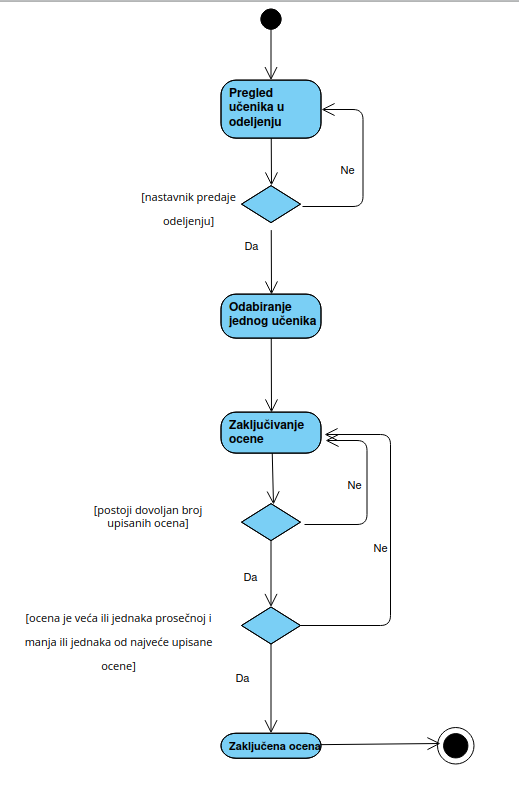
\includegraphics[scale=0.4]{imgs/Dijagram_aktivnosti_nastavnik_zaključuje_ocenu.png}
    \end{center}
\caption{Dijagram aktivnosti Zaključivanje ocene učeniku}
\end{figure}


\newpage
\subsection{Aktivnosti Razrednog starešine}

\subsubsection{Slučaj upotrebe: Razredni starešina opravdava učeniku evidentirani izostanak}
1. \textbf{Kratak opis:} Na osnovu opravdanja koje je učenik dostavio uživo ili elektronski skenirano kroz sistem razredni starešina evidentira izostanak kao opravdan. Sistem čuva promenu statusa odgovarajućeg izostanka i o tome obaveštava razrednog starešinu. \\

2. \textbf{Učesnici:}
\begin{enumerate} [label=(\alph*)]
\item Razredni starešina
\item Učenik
\end{enumerate} 

3. \textbf{Preduslov:} Razredni starešina je registrovani korisnik sistema. Razredni starešina ima pristup Internetu. Sistem je u funkciji. Učenik je dostavio opravdanje. \\

4. \textbf{Postuslov:} Sistem je evidentirao izostanak učenika kao opravdan. Baza je ažurirana. \\

5. \textbf{Osnovni tok:} 
\begin{enumerate} [label=(\alph*)]
\item Razredni starešina pristupa stranici sa listom učenika u svom odeljenju
\item Razredni starešina pritiska na dugme za pristup korisničkom profilu odgovarajućeg učenika
\item Sistem otvara profil učenika
\item Razredni starešina pritiska na dugme za izlistavanje izostanaka učenika
\item Sistem prikazuje listu izostanaka i status svakog izostanka (opravdan/neopravdan)
\item Razredni starešina pritiska odgovarajući neopravdani izostanak
\item Sistem prikazuje dialog box (da/ne) i pita razrednog starešinu da li želi da promeni status neopravdanog izostanka
\item Razredni starešina potvrđuje promenu
\item Sistem čuva promenu statusa izostanka
\item Sistem obaveštava razrednog starešinu o uspešnoj promeni statusa izostanka
\end{enumerate}

6. \textbf{Alternativni tokovi:}
\begin{enumerate} [label=(\roman*)]
\item Razredni starešina ne potvrđuje promenu statusa izostanka - Ako u koraku (h) razredni starešina odgovori odrično ili ugasi dialog box sistem ne evidentira promenu statusa. Proces se nastavlja iz koraka (e). 
\end{enumerate}

7. \textbf{Podtokovi}: - \\

8. \textbf{Specijalni zahtevi}: Izostanak se mora opravdati u roku od dve nedelje nakon evidentiranja. Nakon isteka roka razredni starešina više nema mogućnost opravdavanja i status izostanka ostaje - neopravdan. \\

9. \textbf{Dodatne informacije}: - \\

\begin{figure} [!ht]
    \begin{center}
        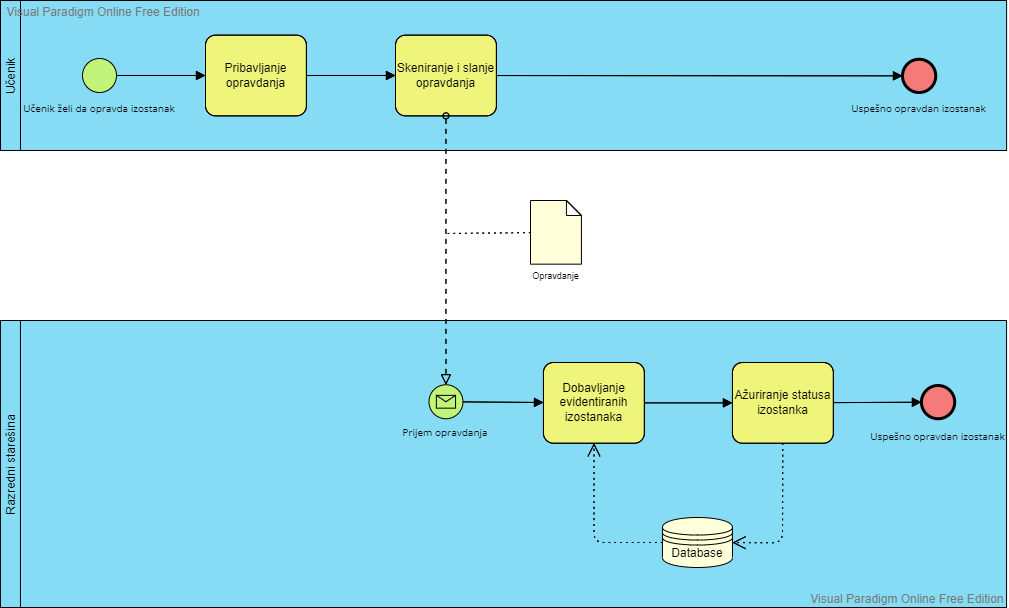
\includegraphics[scale=0.34]{imgs/BPMN_opravdavanje_casova.png}
    \end{center}
\caption{BPMN dijagram saradnje Opravdavanje izostanka učeniku}
\end{figure}

\begin{figure} [!ht]
    \begin{center}
        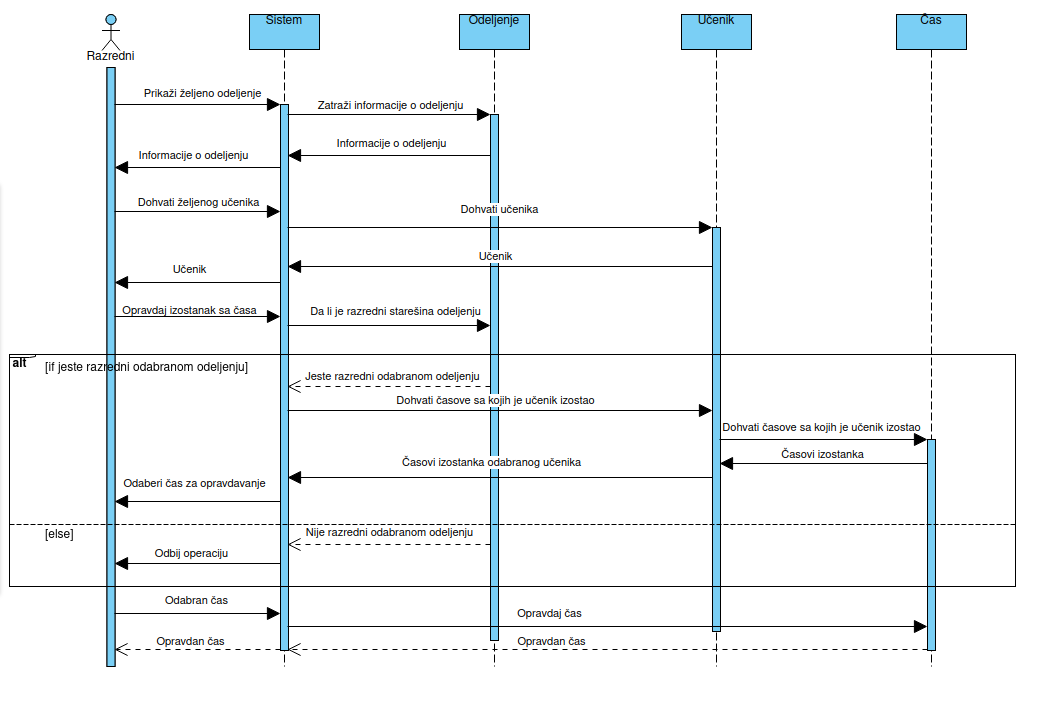
\includegraphics[scale=0.34]{imgs/Dijagram_sekvence_razredni_pravda_cas.png}
    \end{center}
\caption{Dijagram sekvence Opravdavanje izostanka učeniku}
\end{figure}


\newpage
\subsubsection{Slučaj upotrebe: Razredni starešina izriče učeniku lakšu disciplinsku meru}
1. \textbf{Kratak opis:} Na osnovu donesene odluke razredni starešina unosi u sistem lakšu disciplinsku meru izrečenu učeniku. Sistem validira i čuva unete podatke i o tome obaveštava razrednog starešinu. \\

2. \textbf{Učesnici:}
\begin{enumerate} [label=(\alph*)]
\item Razredni starešina
\end{enumerate} 

3. \textbf{Preduslov:} Razredni starešina je registrovani korisnik sistema. Razredni starešina ima pristup Internetu. Sistem je u funkciji. \\

4. \textbf{Postuslov:} Dokument o izrečenoj meri je unet u arhivu dokumenata sistema. Disciplinska mera učenika evidentirana je u sistemu. Baza je ažurirana. \\

5. \textbf{Osnovni tok:} 
\begin{enumerate} [label=(\alph*)]
\item Razredni starešina pristupa stranici sa listom učenika u svom odeljenju
\item Razredni starešina pritiska na dugme za pristup korisničkom profilu odgovarajućeg učenika
\item Sistem otvara profil učenika
\item Razredni starešina pritiska dugme za kreiranje dokumenta o disciplinskoj meri
\item Sistem prikazuje obrazac za kreiranje dokumenta o disciplinskoj meri 
\item Razredni starešina unosi tražene podatke
\item Razredni starešina pritiskom na dugme potvrđuje unos
\item Sistem vrši validaciju podataka
\item Sistem čuva podatke
\item Sistem obaveštava razrednog starešinu o uspešno izrečenoj disciplinskoj meri
\end{enumerate}

6. \textbf{Alternativni tokovi:}
\begin{enumerate} [label=(\roman*)]
\item Razredni starešina unosi nevalidne podatke u obrazac - Ako u koraku (h) sistem utvrdi nevalidno polje obrasca (prazno obavezno polje) sistem obaveštava razrednog starešinu obeležavanjem neispravnog polja. Razredni starešina ispravlja neispravno polje. Proces se nastavlja iz koraka (f).
\end{enumerate}

7. \textbf{Podtokovi}: - \\

8. \textbf{Specijalni zahtevi}: U slučaju ukora odeljenskog veća prethodno je održana sednica na kojoj je disciplinska mere izglasana. \\

9. \textbf{Dodatne informacije}: Obavezna polja obrasca jesu: datum, nivo mere (opomena/ukor razrednog starešine/ukor odeljenskog veća), razlog izricanja mere. Opciono polje je napomena. Lakše disciplinske mere ne povlače smanjenje ocene iz vladanja. Odeljensko veće čine nastavnici koji izvode nastavu u određenom odeljenju. \\

\begin{landscape}
\begin{figure} [!ht]
    \begin{center}
        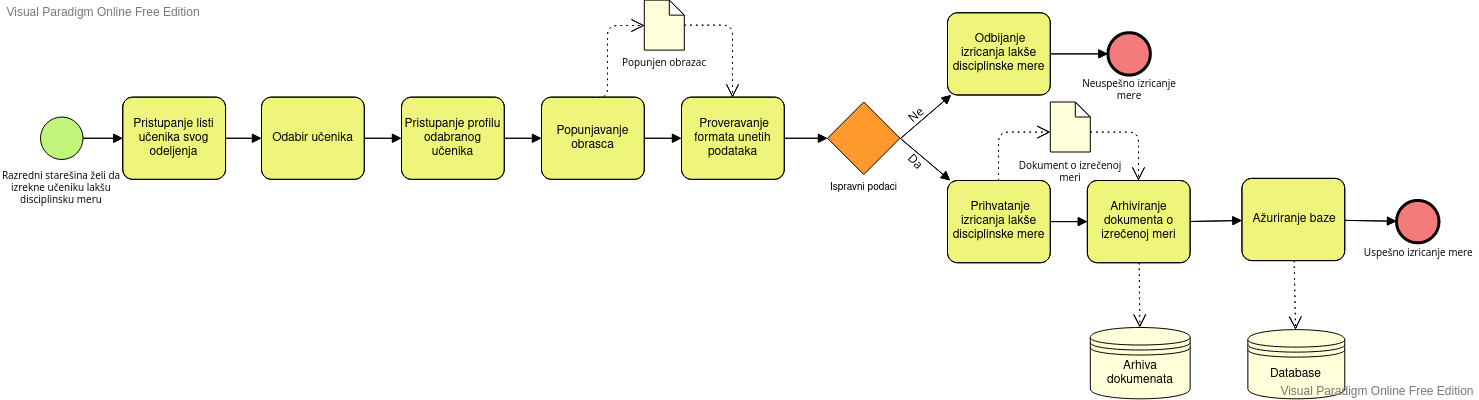
\includegraphics[scale=0.45]{imgs/BPMN_izricanje_lakse_disciplinske_mere.png}
    \end{center}
\caption{BPMN dijagram procesa Izricanje lakše disciplinske mere učeniku}
\end{figure}
\end{landscape}


\newpage
\subsection{Aktivnosti Direktora}

\begin{figure} [!ht]
    \begin{center}
        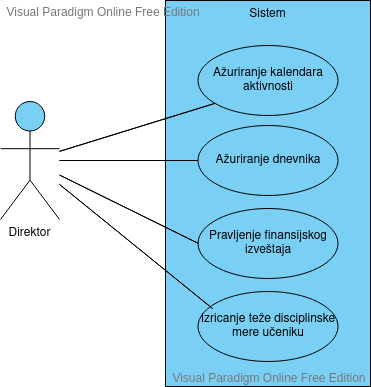
\includegraphics[scale=0.6]{imgs/direktor_use_case.png}
    \end{center}
\caption{Dijagram slučajeva upotrebe Direktora}
\end{figure}

\subsubsection{Slučaj upotrebe: Direktor ažurira kalendar aktivnosti}
1. \textbf{Kratak opis:} Direktor pristupa kalendaru aktivnosti i vrši željenu izmenu. Sistem validira i čuva unete podatke i obaveštava direktora o uspešnoj izmeni kalendara aktivnosti.\\

2. \textbf{Učesnici:}
\begin{enumerate} [label=(\alph*)]
\item Direktor
\end{enumerate} 

3. \textbf{Preduslov:} Direktor je registrovani korisnik sistema. Direktor ima pristup Internetu. Sistem je u funkciji. Kalendar aktivnosti je kreiran. \\

4. \textbf{Postuslov:} U kalendar aktivnosti uneta je željena izmena. Baza je ažurirana. \\

5. \textbf{Osnovni tok:} 
\begin{enumerate} [label=(\alph*)]
\item Direktor pristupa stranici na kojoj je prikazan kalendar aktivnosti
\item Direktor pritiska na dugme ``Izmeni kalendar aktivnosti"  
\item Sistem otvara pogled za ažuriranje kalendara
\item Direktor pritiska na željeni datum u kalendaru
\item Sistem prikazuje direktoru padajući meni sa aktivnostima
\item Direktor odabira željenu aktivnost za taj datum
\item Sistem validira unetu izmenu
\item Sistem čuva izmenu u kalendaru
\item Sistem vraća poruku o uspešnoj izmeni kalendara aktivnosti 
\end{enumerate}

6. \textbf{Alternativni tokovi:}
\begin{enumerate} [label=(\roman*)]
\item Neispunjenost zakonskih uslova - Ukoliko u koraku (g) sistem utvrdi da nakon izmene broj nastavnih dana ne ispunjava zakonski minimum ili premašuje zakonski maksimum, sistem odbija izmenu i o razlogu obaveštava direktora. Proces se nastavlja iz koraka (c).
\end{enumerate}

7. \textbf{Podtokovi}:  - \\

8. \textbf{Specijalni zahtevi}: - \\

9. \textbf{Dodatne informacije}: Moguće aktivnosti za svaki datum su: nastavni dan, nenastavni dan, raspust i državni praznik. Direktor nema opciju da ukloni ili doda državni praznik. \\

\begin{landscape}
\begin{figure} [!ht]
    \begin{center}
        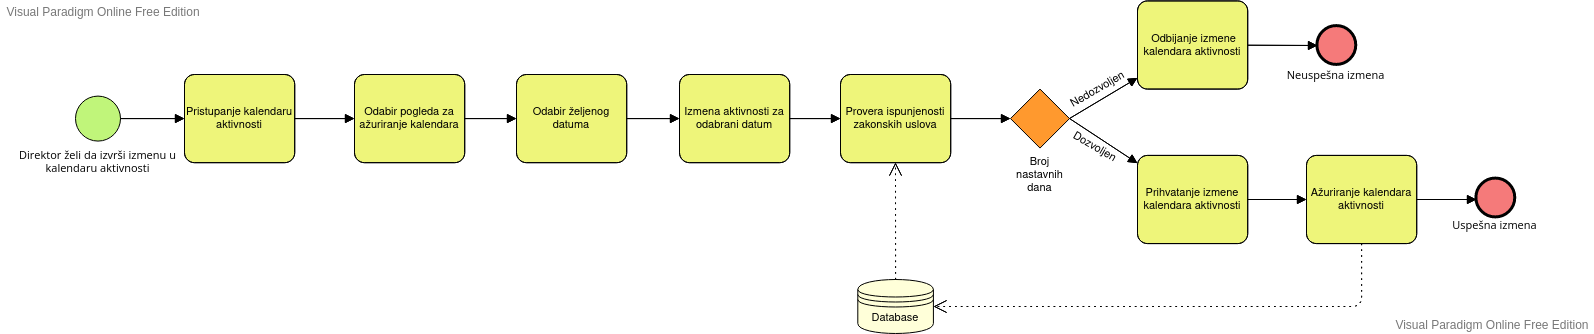
\includegraphics[scale=0.42]{imgs/BPMN_izmena_kalendara.png}
    \end{center}
\caption{BPMN dijagram procesa Ažuriranje kalendara aktivnosti}
\end{figure}
\end{landscape}

\subsubsection{Slučaj upotrebe: Direktor ažurira dnevnik} 
1. \textbf{Kratak opis:} Direktor pristupa elektronskom dnevniku izabranog odeljenja i vrši željenu izmenu. Sistem validira i čuva unete podatke i obaveštava direktora o uspešnoj izmeni dnevnika. \\

2. \textbf{Učesnici:}
\begin{enumerate} [label=(\alph*)]
\item Direktor
\end{enumerate} 

3. \textbf{Preduslov:} Direktor je registrovani korisnik sistema. Direktor ima pristup Internetu. Sistem je u funkciji. \\

4. \textbf{Postuslov:}  U elektronski dnevnik unete su željene izmene. Baza je ažurirana.\\

5. \textbf{Osnovni tok:} 
\begin{enumerate} [label=(\alph*)]
\item Direktor pristupa početnoj strani elektronskog dnevnika
\item Direktor pritiskom na dugme odabira dnevnik željenog odeljenja
\item Sistem prikazuje informacije iz dnevnika tog odeljenja
\item Direktor pritiska na dugme za izmenu
\item Sistem prikazuje direktoru opcije za izmenu
\item Direktor vrši izmenu:
\begin{enumerate} [label=(\roman*)]
    \item Ukoliko direktor izabere opciju ``Izmena ocena'' sistem prebacuje izvršavanje na podtok P1
    \item Ukoliko direktor izabere opciju ``Dodeljivanje razrednog starešine'' sistem prebacuje izvršavanje na podtok P2
    \item Ukoliko direktor izabere opciju ``Pravdanje izostanka'' sistem prebacuje izvršavanje na podtok P3
    \item Ukoliko direktor izabere opciju ``Promeni nastavnika'' sistem prebacuje izvršavanje na podtok P4
\end{enumerate}
\item Sistem vraća poruku o uspešnoj izmeni dnevnika

\end{enumerate}

6. \textbf{Alternativni tokovi:}
\begin{enumerate} [label=(\roman*)]
    \item Direktor ne vrši izmenu - Ako u koraku (f) osnovnog toka direktor izabere opciju ``Nazad'' proces se nastavlja iz koraka (c) osnovnog toka.
    \item Direktor unosi nevalidne podatke u obrazac - Ako u koraku (h) podtoka P1 sistem utvrdi nevalidnu ocenu (ocena nije od 1 do 5) ili prazno obavezno polje obaveštava direktora obeležavanjem neispravnog polja. Direktor ispravlja neispravno polje. Proces se nastavlja iz koraka (f) podtoka P1.
    \item Nastavnik već razredni drugom odeljenju - Ako u koraku (d) podtoka P2 sistem utvrdi da je odabrani nastavnik već dodeljen za razrednog starešinu drugom odeljenju, sistem odbija dodelu i o tome obaveštava direktora. Proces se nastavlja iz koraka (b) podtoka P2.
    \item Direktor ne potvrđuje promenu statusa izostanka - Ako u koraku (f) podtoka P3 direktor odgovori odrično ili ugasi dialog box sistem ne evidentira promenu statusa izostanka. Proces se nastavlja iz koraka (c) podtoka P3.
    \item Direktor pokušava nedozvoljenu zamenu nastavnika - Ako u koraku (f) podtoka P4 sistem utvrdi da bi promenom opterećenost nastavnika koji se menja pala ispod minimalne ili opterećnost nastavnika koji se bira kao zamena premašila maksimalnu dozvoljenu, sistem odbija zamenu i o razlozima obaveštava direktora. Proces se nastavlja iz koraka (a) podtoka P4.
\end{enumerate}

7. \textbf{Podtokovi}: \\
P1: 
\begin{enumerate} [label=(\alph*)]
\item Sistem prikazuje direktoru spisak učenika u odeljenju
\item Direktor pritiska na odabranog učenika
\item Sistem prikazuje sve ocene odabranog učenika
\item Direktor pritiska na ocenu koju želi da izmeni
\item Sistem otvara obrazac sa informacijama o oceni
\item Direktor menja sadržaj obrasca
\item Direktor potvrđuje izmenu ocene
\item Sistem validira unetu izmenu
\item Sistem čuva izmenu u elektronskom dnevniku
\end{enumerate}
P2:
\begin{enumerate} [label=(\alph*)]
\item Sistem prikazuje direktoru spisak nastavnika
\item Direktor pritiska na odabranog nastavnika
\item Direktor potvrđuje dodelu razrednog
\item Sistem validira dodelu
\item Sistem čuva dodelu u elektronskom dnevniku
\end{enumerate}
P3:
\begin{enumerate} [label=(\alph*)]
\item Sistem prikazuje direktoru spisak učenika u odeljenju
\item Direktor pritiska na odabranog učenika
\item Sistem prikazuje listu izostanaka i status svakog izostanka
\item Direktor pritiska na odabrani neopravdani izostanak
\item Sistem prikazuje dialog box (da/ne) i pita direktora da li želi da promeni status neopravadnog izostanka
\item Direktor potvrđuje izmenu
\item Sistem čuva promenu statusa izostana u elektronskom dnevniku
\end{enumerate}
P4:
\begin{enumerate} [label=(\alph*)]
\item Sistem prikazuje direktoru spisak nastavnika koji predaju datom odeljenju po predmetima
\item Direktor pritiska na odabrani predmet za koji želi da promeni nastavnika
\item Sistem prikazuje spisak nastavnika zaposlenih u školi koji predaju taj predmet
\item Direktor pritiska na nastavnika zaposlenog u školi kojeg bira kao zamenu
\item Direktor potvrđuje promenu 
\item Sistem validira promenu
\item Sistem čuva promenu u elektronskom dnevniku
\end{enumerate}

8. \textbf{Specijalni zahtevi}: U slučaju izmene ocene učenika direktor je prethodno utvrdio sa predmetnim nastavnikom da je došlo do greške prilikom upisa ocene. \\

9. \textbf{Dodatne informacije}: Minimalna i maksimalna opterećenost nastavnika definisane su pravilnikom škole. Nastavnik može biti razredni starešina samo jednom odeljenju. Obrazac sadrži informacije o oceni: ocena, tip (kontrolni/pismeni/usmeni/aktivnost). Opciono polje je napomena. \\


\begin{figure} [!ht]
    \begin{center}
        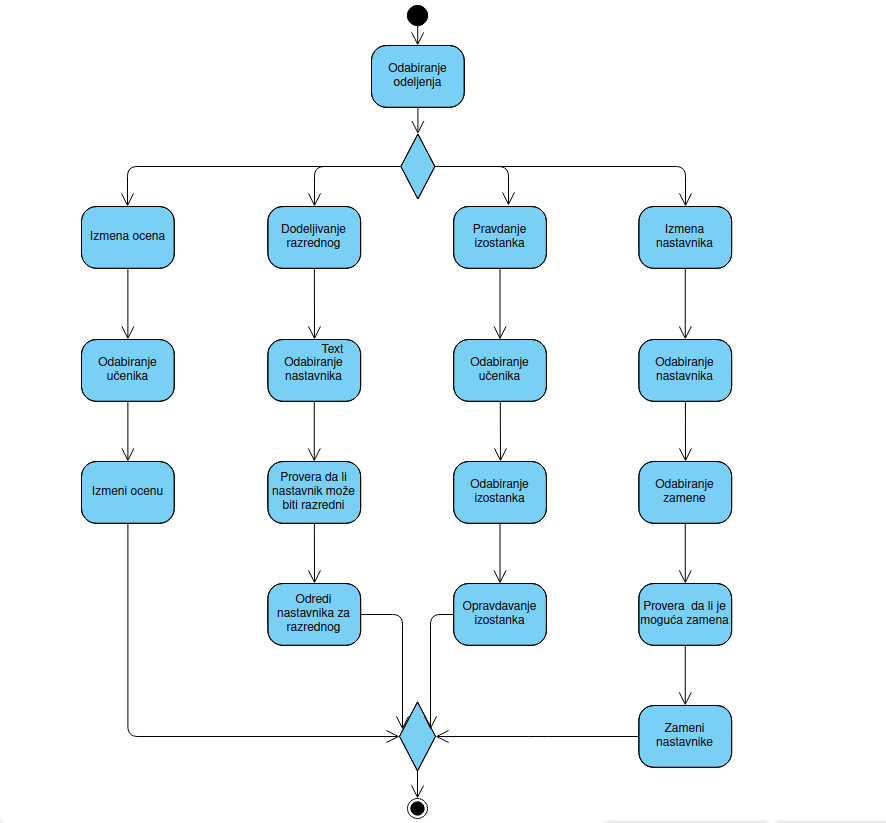
\includegraphics[scale=0.4]{imgs/Dijagram_aktivnosti_direktor_azurira_dnevnik.png}
    \end{center}
\caption{Dijagram aktivnosti Ažuriranje dnevnika}
\end{figure}

\newpage
\subsubsection{Slučaj upotrebe: Direktor pravi finansijski izveštaj škole}
1. \textbf{Kratak opis:} Direktor na osnovu finansijskih prihoda i rashoda pravi finansijski izveštaj škole. Sistem validira i čuva unete podatke i obaveštava direktora o uspešno unetom izveštaju. \\

2. \textbf{Učesnici:}
\begin{enumerate} [label=(\alph*)]
\item Direktor
\end{enumerate} 

3. \textbf{Preduslov:} Direktor je registrovani korisnik sistema. Direktor ima pristup Internetu. Sistem je u funkciji. \\

4. \textbf{Postuslov:} Finansijski izveštaj unet je u arhivu dokumenata sistema. \\

5. \textbf{Osnovni tok:} 
\begin{enumerate} [label=(\alph*)]
\item Direktor pristupa stranici sa finansijskim izveštajima
\item Direktor pritiska dugme za kreiranje novog izveštaja
\item Sistem kreira prazan finansijski izveštaj
\item Direktor pritiska dugme za dodavanje nove transakcije u izveštaj
\item Sistem prikazuje formular za unošenje informacija o novoj transakciji
\item Direktor unosi informacije o transakciji
\item Direktor pritiskom na dugme potvrđuje unos
\item Sistem vrši validaciju podataka
\item Sistem upisuje datu transakciju
\item Sistem prikazuje ažuriran finansijski izveštaj\footnote{Koraci (d), (e), (f), (g), (h), (i), (j) ponavljaju se sve dok ima transakcija koje je potrebno zavesti u izveštaj}
\item Direktor pritiska dugme za zaključivanje izveštaja
\item Sistem čuva podatke
\item Sistem vraća poruku o uspešno kreiranom izveštaju

\end{enumerate}

6. \textbf{Alternativni tokovi:} 
\begin{enumerate} [label=(\roman*)]
\item Direktor unosi nevalidne podatke u formular - Ako u koraku (h) sistem utvrdi neispravno polje formulara, sistem obaveštava direktora obeležavanjem nevalidnog polja. Direktor ispravlja neispravno polje. Proces se nastavlja iz koraka (f).
\item Direktor uklanja transakciju iz izveštaja - Ukoliko u koraku (j) direktor utvrdi da je u izveštaj uneo pogrešnu transakciju, klikom bira opciju za uklanjanje te transakcije nakon čega sistem ažurira izveštaj. Proces se nastavlja iz koraka (j).  
\end{enumerate}

7. \textbf{Podtokovi}:  - \\

8. \textbf{Specijalni zahtevi}: - \\

9. \textbf{Dodatne informacije}: Obavezna polja formulara jesu: datum, tip transakcije (priliv/odliv), iznos. Opciono polje je napomena. Ovaj slučaj upotrebe služi samo za dokumentovanje transakcija, ne i za njihovo obavljanje. Finansijski izveštaj pravi se na mesečnom nivou.  \\

\begin{figure} [!ht]
    \begin{center}
        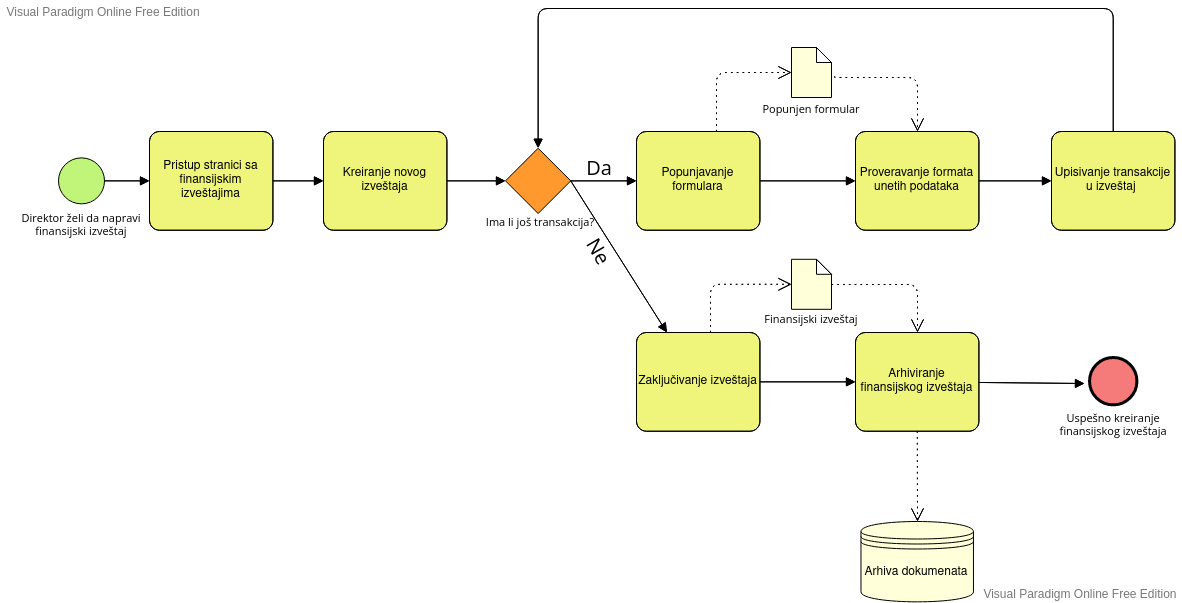
\includegraphics[scale=0.37]{imgs/BPMN_pravljenje_finansijskog_izvestaja.png}
    \end{center}
\caption{BPMN dijagram procesa Pravljenje finansijskog izveštaja}
\end{figure}


\subsubsection{Slučaj upotrebe: Direktor izriče učeniku težu disciplinsku meru}
1. \textbf{Kratak opis:} Na osnovu donesene odluke direktor unosi u sistem težu disciplinsku meru izrečenu učeniku. Sistem validira i čuva unete podatke i o tome obaveštava direktora. \\

2. \textbf{Učesnici:}
\begin{enumerate} [label=(\alph*)]
\item Direktor
\end{enumerate} 

3. \textbf{Preduslov:} Direktor je registrovani korisnik sistema. Direktor ima pristup Internetu. Sistem je u funkciji. \\

4. \textbf{Postuslov:} Dokument o izrečenoj meri je unet u arhivu dokumenata sistema. Disciplinska mera učenika evidentirana je u sistemu. Baza je ažurirana. \\

5. \textbf{Osnovni tok:} 
\begin{enumerate} [label=(\alph*)]
\item Direktor pristupa stranici sa listom svih učenika podeljenih po razredima i odeljenjima 
\item Direktor pritiska na dugme za pristup korisničkom profilu odgovarajućeg učenika
\item Sistem otvara profil učenika
\item Direktor pritiska dugme za kreiranje dokumenta o disciplinskoj meri
\item Sistem prikazuje obrazac za kreiranje dokumenta o disciplinskoj meri 
\item Direktor unosi tražene podatke
\item Direktor pritiskom na dugme potvrđuje unos
\item Sistem vrši validaciju podataka
\item Sistem čuva podatke
\item Sistem obaveštava direktora o uspešno izrečenoj disciplinskoj meri
\end{enumerate}

6. \textbf{Alternativni tokovi:}
\begin{enumerate} [label=(\roman*)]
\item Direktor unosi nevalidne podatke u obrazac - Ako u koraku (h) sistem utvrdi nevalidno polje obrasca (prazno obavezno polje) sistem obaveštava direktora obeležavanjem neispravnog polja. Direktor ispravlja neispravno polje. Proces se nastavlja iz koraka (f).
\end{enumerate}

7. \textbf{Podtokovi}: - \\

8. \textbf{Specijalni zahtevi}: Roditelj ili staratelj upoznat je sa disciplinskim postupkom koji se vodi protiv učenika. U slučaju ukora nastavničkog veća ili isključenja iz škole prethodno je održana sednica nastavičkog veća na kojoj je disciplinska mere izglasana. \\

9. \textbf{Dodatne informacije}: Obavezna polja obrasca jesu: datum, nivo mere (ukor direktora/ukor nastavničkog veća/isključenje učenika iz škole), razlog izricanja mere. Opciono polje je napomena. Teže disciplinske mere povlače smanjenje ocene iz vladanja (ukor direktora na 4 ili 3, ukor nastavničkog veća na 2, isključenje iz škole na 1). Nastavničko veće čine svi nastavnici zaposleni u školi. U slučaju isključenja učenika iz škole administrator će deaktivirati nalog učenika. \\


\begin{landscape}
\begin{figure} [!ht]
    \begin{center}
        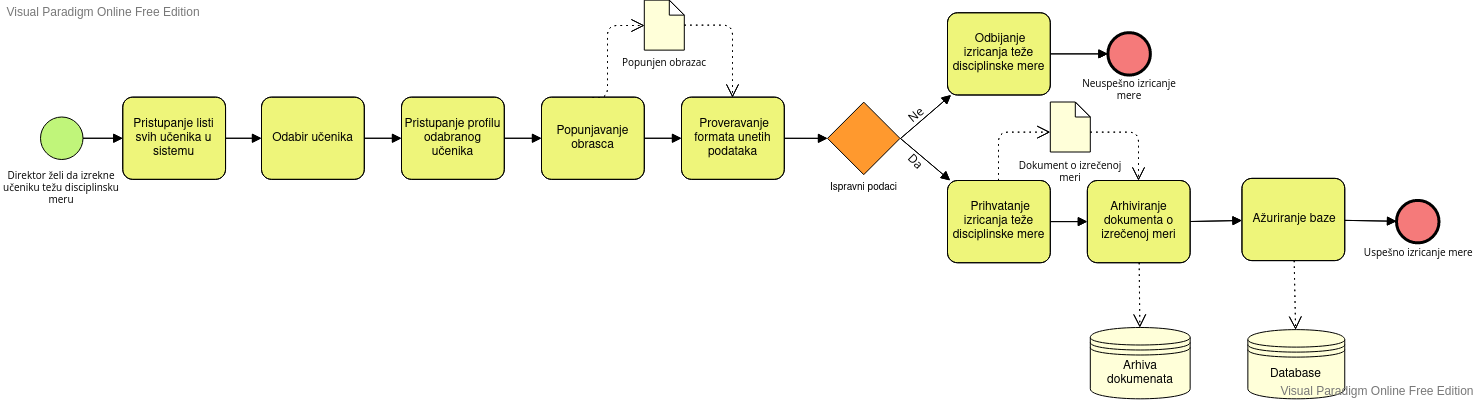
\includegraphics[scale=0.45]{imgs/BPMN_izricanje_teze_disciplinske_mere.png}
    \end{center}
\caption{BPMN dijagram procesa Izricanje teže disciplinske mere učeniku}
\end{figure}
\end{landscape}


\newpage
\subsection{Aktivnosti Administratora}

\begin{figure} [!ht]
    \begin{center}
        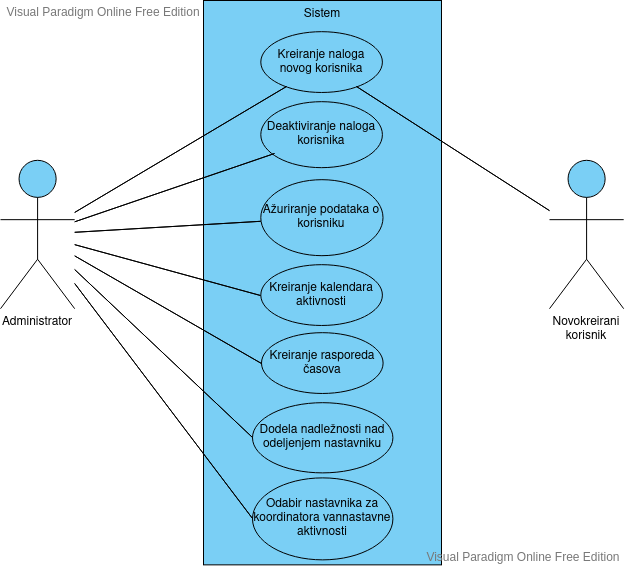
\includegraphics[scale=0.5]{imgs/admin_use_case.png}
    \end{center}
\caption{Dijagram slučajeva upotrebe Administratora sistema}
\end{figure}


\subsubsection{Slučaj upotrebe: Administrator kreira nalog novog korisnika} 
1. \textbf{Kratak opis:} Administrator pravi profil za novog korisnika sistema (nastavnika ili učenika). Sistem validira podatke i vraća potvrdu o uspešno kreiranom korisniku. Korisnik se prijavljuje na sistem i kreira svoju lozinku. \\

2. \textbf{Učesnici:}
\begin{enumerate} [label=(\alph*)]
\item Administrator
\item Novokreirani korisnik
\end{enumerate} 

3. \textbf{Preduslov:} Administrator je korisnik sistema. Administrator ima pristup Internetu. Administrator ima potpisano ovlašćenje direktora za kreiranje naloga korisniku. Korisnik ima pristup Internetu. Sistem je u funkciji. \\

4. \textbf{Postuslov:} Novi korisnik je kreiran i ima pristup sistemu. Baza je ažurirana. \\

5. \textbf{Osnovni tok:} 
\begin{enumerate} [label=(\alph*)]
\item Administrator pristupa stranici za kreiranje novog korisnika
\item Sistem prikazuje opcije za kreiranje novog korisnika
\item Administrator bira tip korisnika koji se kreira:
\begin{enumerate} [label=(\roman*)]
    \item Ukoliko administrator odabere opciju da se kreira nastavnički profil sistem prebacuje izvršavanje na podtok P1
    \item Ukoliko administrator odabere opciju da se kreira učenički profil sistem prebacuje izvršavanje na podtok P2
\end{enumerate}
\item Administrator potvrđuje unete podatke pritiskom na dugme
\item Sistem validira podatke
\item Sistem kreira novog korisnika
\item Administrator šalje e-mail sa linkom za pristup sistemu novokreiranom korisniku
\item Novokreirani korisnik pristupa sistemu preko linka poslatog e-mailom
\item Korisnik prilikom prvog pristupa sistemu postavlja svoju lozinku
\item Korisnik potvrđuje postavljanje lozinke
\item Sistem vrši validaciju formata lozinke
\item Sistem postavlja lozinku korisnika
\item Sistem obaveštava korisnika o uspešnom postavljanju lozinke
\item Sistem obaveštava administratora da je nalog kreiran
\end{enumerate}

6. \textbf{Alternativni tokovi:}
\begin{enumerate} [label=(\roman*)]
\item Administrator unosi nevalidne podatke u formular - Ako u koraku (e) glavnog toka sistem utvrdi neispravno polje formulara (prazno obavezno polje ili u sistemu već postoji korisnik sa istim JMBG), sistem obaveštava administratora obeležavanjem nevalidnog polja. Administrator ispravlja neispravno polje. Proces se nastavlja iz koraka (d) glavnog toka.
\item Novokreiranom korisniku nije stigao e-mail - Ukoliko u koraku (h) glavnog toka korisnik utvrdi da mu nije stigao e-mail, zahteva ponovno slanje istog. Proces se nastavlja iz koraka (g) glavnog toka.
\item Neispravan format lozinke - Ako u koraku (k) glavnog toga sistem utvdi da se pokušava postavljanje kratke ili nedovoljno bezbedne lozinke, sistem odbija postavljanje lozinke i o tome obaveštava korisnika. Korisnik ispravlja lozinku. Proces se nastavlja iz koraka (i) glavnog toka.
\end{enumerate}

7. \textbf{Podtokovi}: \\
P1:
\begin{enumerate} [label=(\alph*)]
\item Administrator popunjava formular za kreiranje nastavnika
\end{enumerate}
P2:
\begin{enumerate} [label=(\alph*)]
\item Administrator popunjava formular za kreiranje učenika
\end{enumerate}

8. \textbf{Specijalni zahtevi}: - \\

9. \textbf{Dodatne informacije}: Obavezna polja formulara za kreiranje nastavnika su: ime, prezime, JMBG, e-mail adresa, broj telefona, obrazovanje, predmet koji predaje i prethodno radno iskustvo. Obavezna polja formulara za kreiranje učenika su: ime, prezime, JMBG, e-mail adresa, broj telefona, broj telefona roditelja, dosadašnje školovanje. Lozinka ne sme biti kraća od 8 karaktera, mora sadržati bar jedno slovo i bar jednu cifru. \\

\begin{landscape}
\begin{figure} [!ht]
    \begin{center}
        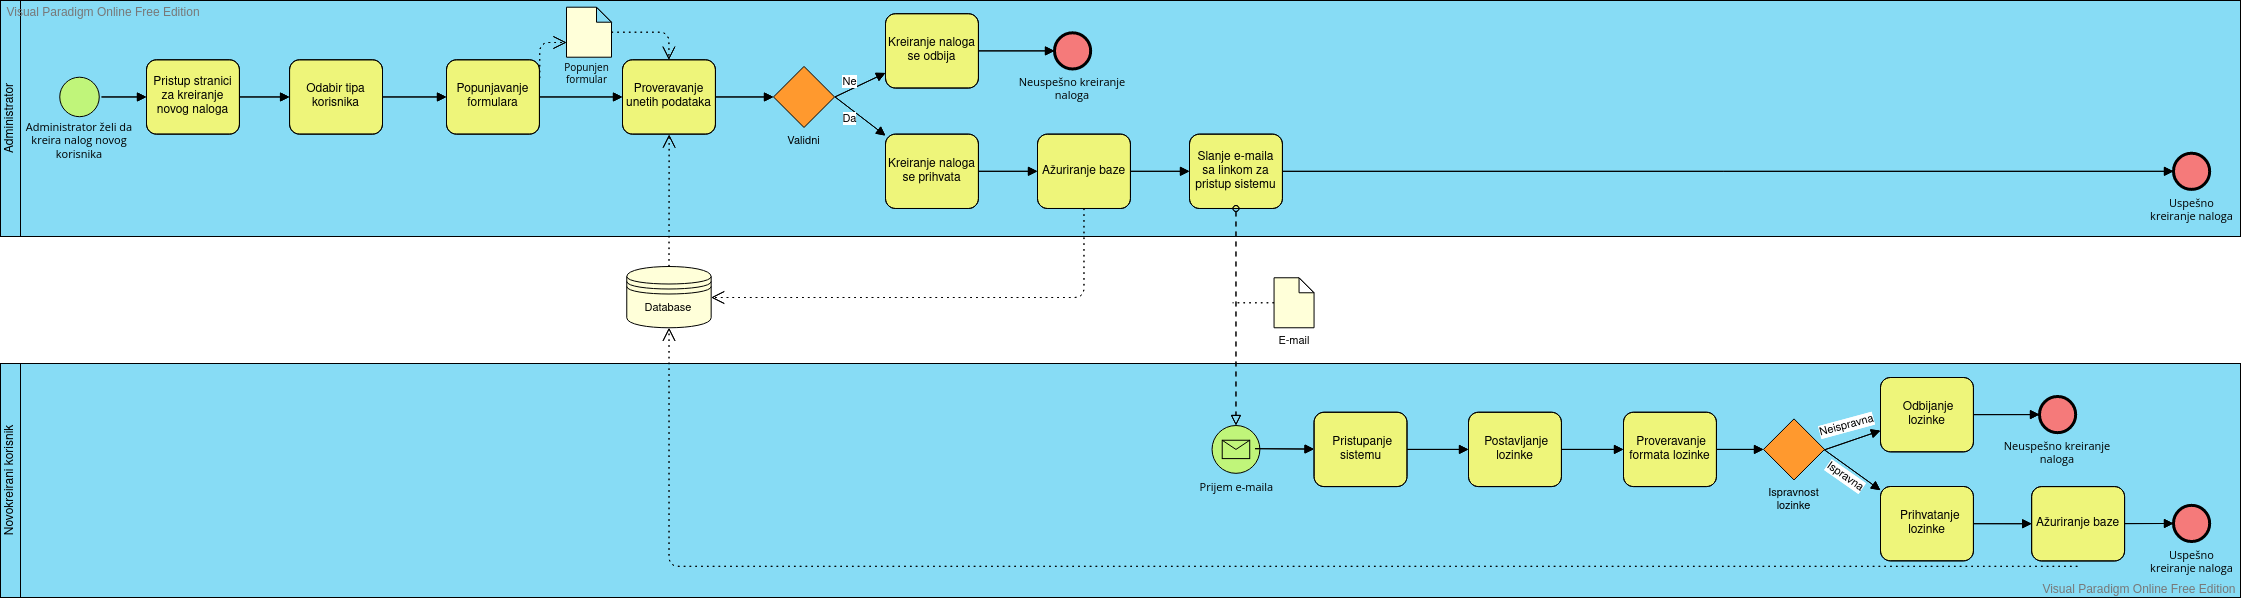
\includegraphics[scale=0.28]{imgs/BPMN_kreiranje_korisnika.png}
    \end{center}
\caption{BPMN dijagram saradnje Kreiranje naloga novog korisnika}
\end{figure}
\end{landscape}


\subsubsection{Slučaj upotrebe: Administrator deaktivira nalog korisnika}
1. \textbf{Kratak opis:} Administrator deaktivira profil korisnika sistema (nastavnika ili učenika). Sistem označava profil korisnika kao neaktivan, onemogućava buduće logovanje korisnika na sistem i obaveštava administratora o uspešnoj deaktivaciji naloga. \\

2. \textbf{Učesnici:}
\begin{enumerate} [label=(\alph*)]
\item Administrator
\end{enumerate} 

3. \textbf{Preduslov:} Administrator je korisnik sistema. Administrator ima pristup Internetu. Administrator ima potpisano ovlašćenje direktora za deaktiviranje naloga korisnika. Sistem je u funkciji. \\

4. \textbf{Postuslov:} Nalog korisnika je deaktiviran i on više nema pristup sistemu. Baza je ažurirana. \\

5. \textbf{Osnovni tok:} 
\begin{enumerate} [label=(\alph*)]
\item Administrator otvara stranicu sa listom korisnika sistema
\item Administrator pritiska dugme za deaktiviranje naloga kod odgovarajućeg korisnika
\item Sistem prikazuje dialog box (da/ne) i pita administratora da li želi da deaktivira nalog korisnika
\item Administrator potvrđuje deaktivaciju naloga korisnika
\item Sistem označava nalog odabranog korisnika kao neaktivan
\item Sistem obaveštava administratora da je nalog uspešno deaktiviran
\end{enumerate}

6. \textbf{Alternativni tokovi:}
\begin{enumerate} [label=(\roman*)]
    \item Administrator ne potvrđuje deaktivaciju - Ako u koraku (d) administrator odgovori odrično ili ugasi dialog box sistem ne deaktivira nalog korisnika. Proces se nastavlja iz koraka (a).
\end{enumerate}

7. \textbf{Podtokovi}: - \\

8. \textbf{Specijalni zahtevi}: - \\

9. \textbf{Dodatne informacije}: - \\


\begin{figure} [!ht]
    \begin{center}
        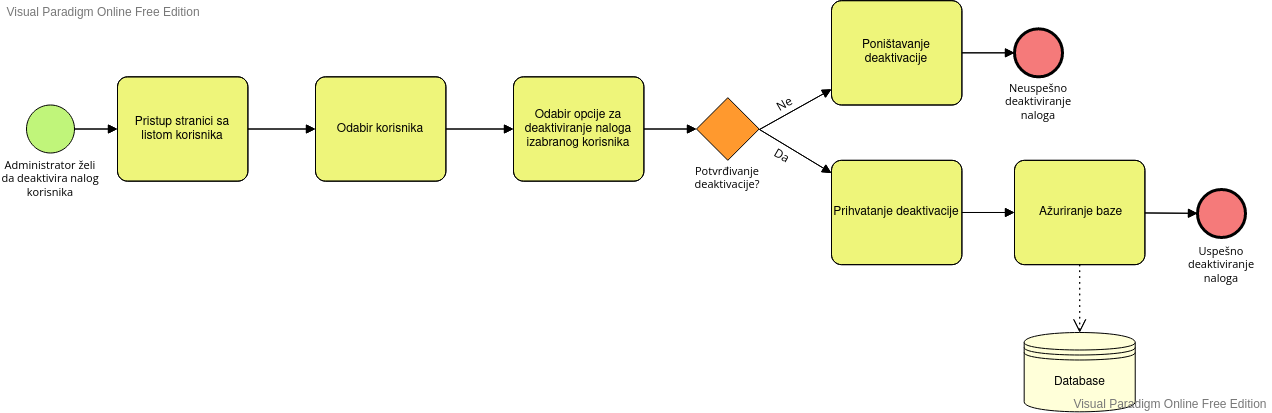
\includegraphics[scale=0.35]{imgs/BPMN_deaktivacija_naloga.png}
    \end{center}
\caption{BPMN dijagram proces Deaktiviranje naloga korisnika}
\end{figure}



\subsubsection{Slučaj upotrebe: Administrator ažurira podatke o korisniku}
1. \textbf{Kratak opis:} Administrator pristupa stranici korisnika i ažurira podatke o odabranom korisniku. Sistem validira i čuva izmene i obaveštava administratora o uspešnom ažuriranju podataka. \\

2. \textbf{Učesnici:}
\begin{enumerate} [label=(\alph*)]
\item Administrator
\end{enumerate} 

3. \textbf{Preduslov:} Administrator je korisnik sistema. Administrator ima pristup Internetu. Poznato je koji podatak o korisniku treba izmeniti i nova vrednost istog. Administrator ima potpisano ovlašćenje direktora za izmenu podataka o korisniku. Sistem je u funkciji. \\

4. \textbf{Postuslov:} Podaci o odabranom korisniku su izmenjeni. Baza je ažurirana. \\

5. \textbf{Osnovni tok:} 
\begin{enumerate} [label=(\alph*)]
\item Administrator otvara stranicu sa listom korisnika sistema
\item Administrator pritiska dugme za ažuriranje podataka kod odgovarajućeg korisnika
\item Sistem otvara stranicu sa korisničkim podacima
\item Administrator menja željeni podatak
\item Sistem prikazuje dialog box (da/ne) i pita administratora da li želi da izvrši promenu
\item Administrator potvrđuje ažuriranje korisničkih podataka
\item Sistem validira izmenu
\item Sistem čuva podatke
\item Sistem obaveštava administratora da su podaci uspešno ažurirani
\end{enumerate}

6. \textbf{Alternativni tokovi:}
\begin{enumerate} [label=(\roman*)]
    \item Administrator ne potvrđuje promenu - Ako u koraku (f) administrator odgovori odrično ili ugasi dialog box sistem ne ažurira korisničke podatke. Proces se nastavlja iz koraka (c).
    \item Nevalidna izmena podataka - Ako u koraku (g) sistem utvrdi da je izmena nevalidna (obavezan podatak se postavlja na prazan), sistem odbija izmenu i o tome obaveštava administratora. Proces se nastavlja iz koraka (c).
\end{enumerate}

7. \textbf{Podtokovi}: - \\

8. \textbf{Specijalni zahtevi}: - \\

9. \textbf{Dodatne informacije}: Podaci o korisniku uneti su u sistem prilikom kreiranja naloga. Sistem onemogućuje izmenu JMBG korisnika. \\


\begin{figure} [!ht]
    \begin{center}
        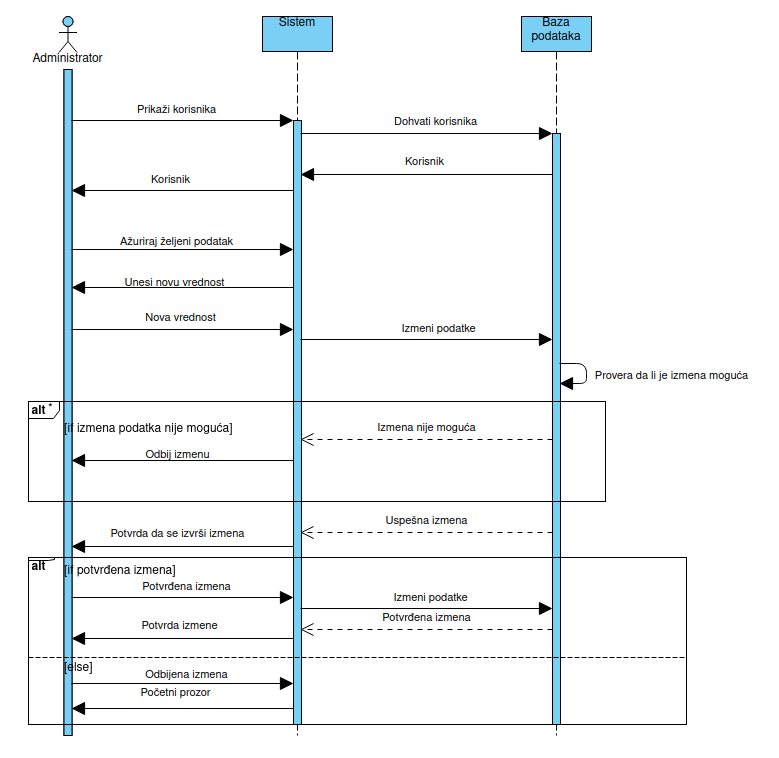
\includegraphics[scale=0.4]{imgs/Dijagram_sekvence_administrator_azurira_podatke.png}
    \end{center}
\caption{Dijagram sekvence Ažuriranje podataka o korisniku}
\end{figure}


\newpage
\subsubsection{Slučaj upotrebe: Administrator kreira kalendar aktivnosti}
1. \textbf{Kratak opis:} Pre početka školske godine administrator pristupa kalendaru i popunjava ga aktivnostima za svaki datum do kraja školske godine u skladu sa planom rada škole. Sistem validira i čuva unete podatke. Sistem obaveštava administratora o uspešnom kreiranju kalendara aktivnosti. \\ 

2. \textbf{Učesnici:}
\begin{enumerate} [label=(\alph*)]
\item Administrator
\end{enumerate} 

3. \textbf{Preduslov:} Administrator je registrovani korisnik sistema. Administrator ima pristup Internetu. Administrator ima plan rada škole potpisan od strane direktora. Sistem je u funkciji. \\

4. \textbf{Postuslov:} Kalendar aktivnosti je kreiran i vidljiv svim korisnicima sistema. Baza je ažurirana. \\

5. \textbf{Osnovni tok:} 
\begin{enumerate} [label=(\alph*)]
\item Administrator pristupa kalendaru
\item Administrator pritiska na određeni datum za koji želi da unese aktivnost
\item Sistem prikazuje administratoru padajući meni sa aktivnostima
\item Administrator odabira željenu aktivnost za taj datum\footnote{Koraci (b), (c), (d) ponavljaju se sve dok se ne popuni kalendar aktivnosti}
\item Sistem validira kalendar aktivnosti
\item Sistem čuva kalendar aktivnosti
\item Sistem vraća poruku o uspešnom kreiranju kalendara aktivnosti
\end{enumerate}

6. \textbf{Alternativni tokovi:}
\begin{enumerate} [label=(\roman*)]
\item Neispunjenost zakonskih uslova - Ukoliko u koraku (e) sistem utvrdi da kreirani kalendar ne ispunjava zakonski minimum ili premašuje zakonski maksimum broja nastavnih dana, sistem ne prihvata kreiranje kalendara i o razlozima obaveštava administratora. Proces se nastavlja iz koraka (b).
\end{enumerate}

7. \textbf{Podtokovi}:  - \\

8. \textbf{Specijalni zahtevi}: - \\

9. \textbf{Dodatne informacije}: Moguće aktivnosti za svaki datum su: nastavni dan, nenastavni dan, raspust i državni praznik. Prilikom unošenja aktivnosti administrator može selektovati više uzastopnih datuma i za njih odjednom odabrati aktivnost. \\

\begin{figure} [!ht]
    \begin{center}
        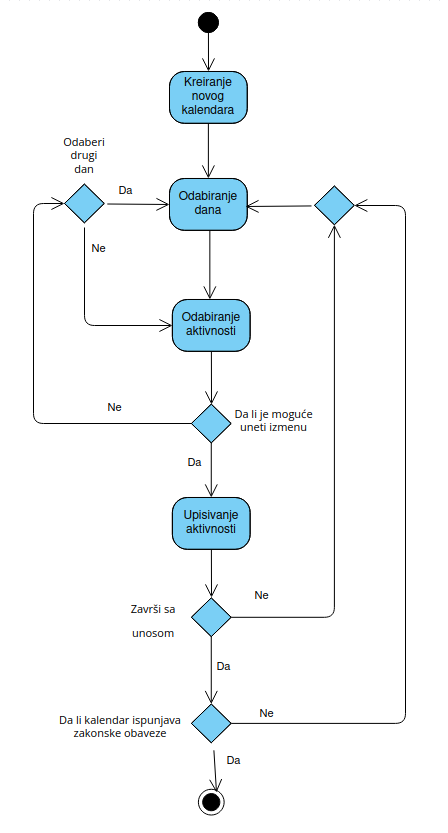
\includegraphics[scale=0.35]{imgs/Dijagram_aktivnosti_administrator_kreira_kalendar.png}
    \end{center}
\caption{Dijagram aktivnosti Kreiranje kalendara aktivnosti}
\end{figure}


\newpage
\subsubsection{Slučaj upotrebe: Administrator kreira raspored časova}
1. \textbf{Kratak opis:} Na početku školske godine u dogovoru sa direktorom i nastavnicima administrator unosi raspored časova za radnu nedelju u sistem. Sistem validira i čuva unete podatke. Sistem obaveštava administratora o uspešno kreiranom rasporedu časova. \\ 

2. \textbf{Učesnici:}
\begin{enumerate} [label=(\alph*)]
\item Administrator
\end{enumerate} 

3. \textbf{Preduslov:} Administrator je registrovani korisnik sistema. Administrator ima pristup Internetu. Administrator ima raspored časova potpisan od strane direktora. Sistem je u funkciji. \\

4. \textbf{Postuslov:} Raspored časova je kreiran i vidljiv svim korisnicima sistema. Baza je ažurirana. \\

5. \textbf{Osnovni tok:} 
\begin{enumerate} [label=(\alph*)]
\item Administrator pristupa stranici za kreiranje rasporeda časova
\item Sistem prikazuje stranicu sa terminima u radnoj nedelji podeljenim po danima
\item Administrator pritiska na odabrani termin
\item Sistem otvara formular za upis podataka o času koji se dodaje u raspored u odabranom terminu
\item Administrator popunjava formular odgovarajućim podacima
\item Administrator potvđuje dodavanje časa 
\item Sistem validira unete podatke\footnote{Koraci (b), (c), (d), (e), (f), (g) ponavljaju se sve dok se ne ispuni fond časova}
\item Sistem vrši proveru da li je došlo do preklapanja u rasporedu časova
\item Sistem čuva raspored časova
\item Sistem vraća poruku o uspešnom kreiranju rasporeda časova
\end{enumerate}

6. \textbf{Alternativni tokovi:}
\begin{enumerate} [label=(\roman*)]
\item Administrator unosi nevalidne podatke u formular - Ako u koraku (g) sistem utvrdi nevalidne podatke (obavezna polja ostala nepopunjena) obaveštava administratora obeležavanjem neispravnog polja. Administrator ispravlja neispravno polje. Proces se nastavlja iz koraka (e).
\item U rasporedu postoje preklapanja - Ako u koraku (h) sistem utvrdi da postoje preklapanja u rasporedu časova, sistem odbija kreiranje rasporeda i obaveštava administratora ispisivanjem časova koji se preklapaju. Proces se nastavlja iz koraka (b).
\end{enumerate}

7. \textbf{Podtokovi}: - \\

8. \textbf{Specijalni zahtevi}: - \\

9. \textbf{Dodatne informacije}: Obavezna polja formulara su: naziv predmeta ili vannastavne aktivnosti, nastavnik, odeljenje i broj kabineta. Opciono polje je napomena. \\


\begin{figure} [!ht]
    \begin{center}
        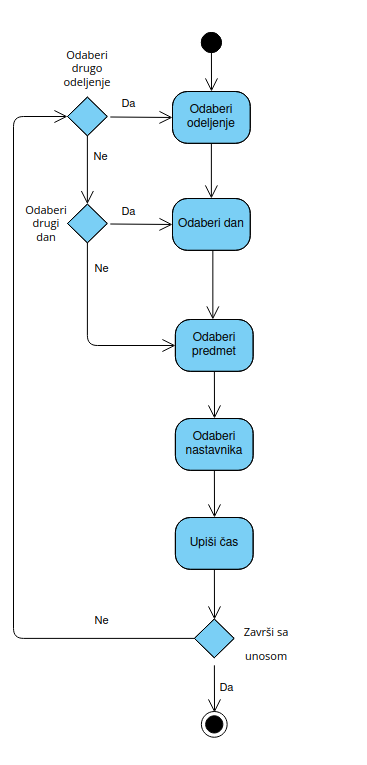
\includegraphics[scale=0.35]{imgs/Dijagram_aktivnosti_administrator_pravi_raspored_casova.png}
    \end{center}
\caption{Dijagram aktivnosti Kreiranje rasporeda časova}
\end{figure}

\newpage
\subsubsection{Slučaj upotrebe: Administrator dodeljuje nadležnost nad odeljenjem nastavniku}
1. \textbf{Kratak opis:} Administrator pristupa korisničkom profilu nastavnika i daje mu nadležnost za držanje nastave iz svog predmeta određenom odeljenju. Sistem validira i čuva izmene i obaveštava administratora o uspešno dodatoj nadležnosti. \\

2. \textbf{Učesnici:}
\begin{enumerate} [label=(\alph*)]
\item Administrator
\end{enumerate} 

3. \textbf{Preduslov:} Administrator je korisnik sistema. Administrator ima pristup Internetu. Administrator ima potpisano ovlašćenje direktora za dodelu nadležnosti nastavniku. Sistem je u funkciji. \\

4. \textbf{Postuslov:} Nastavniku je dodeljena nadležnost nad odeljenjem. Baza je ažurirana. \\

5. \textbf{Osnovni tok:} 
\begin{enumerate} [label=(\alph*)]
\item Administrator pristupa stranici sa listom nastavnika podeljenih po predmetima koji predaju
\item Administrator pritiska na odabranog nastavnika
\item Sistem prikazuje korisnički profil nastavnika
\item Administrator pritiska na dugme ``Dodeli odeljenje''
\item Sistem prikazuje spisak odeljenja kojima nije dodeljen nastavnik iz odgovarajućeg predmeta
\item Administrator pritiskom na dugme bira odeljenje koje dodeljuje nastavniku
\item Sistem validira dodelu nadležnosti
\item Sistem čuva dodelu nadležnosti
\item Sistem obaveštava administratora o uspešnoj dodeli nadležnosti
\end{enumerate}

6. \textbf{Alternativni tokovi:}
\begin{enumerate} [label=(\roman*)]
    \item Administrator pokušava nedozvoljenu dodelu nadležnosti - Ako u koraku (g) sistem utvrdi da bi dodelom nadležnosti opterećnost nastavnika premašila maksimalnu dozvoljenu, sistem odbija dodelu i o razlozima obaveštava administratora. Proces se nastavlja iz koraka (c).
\end{enumerate}

7. \textbf{Podtokovi}: - \\

8. \textbf{Specijalni zahtevi}: - \\

9. \textbf{Dodatne informacije}: Maksimalna opterećenost nastavnika definisana je pravilnikom škole. Dodeljene nadležnosti nastavnicima uzimaju se u obzir kao kriterijum prilikom pravljenja rasporeda časova. \\

\begin{landscape}
\begin{figure} [!ht]
    \begin{center}
        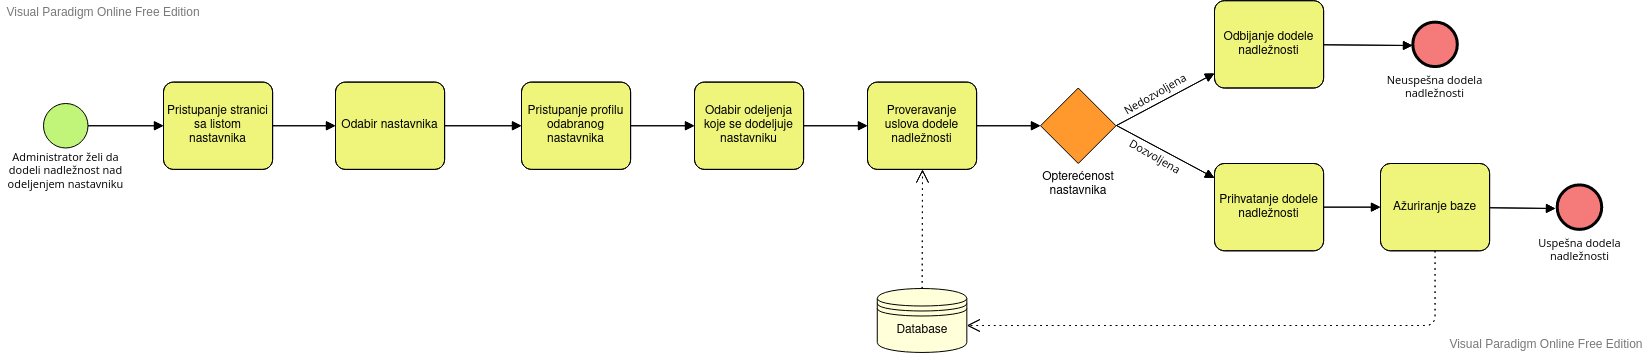
\includegraphics[scale=0.4]{imgs/BPMN_dodela_nadleznosti.png}
    \end{center}
\caption{BPMN dijagram procesa Dodela nadležnosti nad odeljenjem nastavniku}
\end{figure}
\end{landscape}

\subsubsection{Slučaj upotrebe: Administrator odabira nastavnika za koordinatora vannastavne aktivnosti}
1. \textbf{Kratak opis:} Administrator pristupa korisničkom profilu nastavnika i proglašava ga za koordinatora odabrane vannastavne aktivnosti. Sistem validira i čuva izmene i obaveštava administratora o uspešno odabranom koordinatoru. \\

2. \textbf{Učesnici:}
\begin{enumerate} [label=(\alph*)]
\item Administrator
\end{enumerate} 

3. \textbf{Preduslov:} Administrator je korisnik sistema. Administrator ima pristup Internetu. Nastavnik se prijavio za poziciju koordinatora odabrane aktivnosti. Administrator ima potpisano ovlašćenje direktora za odabir nastavnika za koordinatora. Sistem je u funkciji. \\

4. \textbf{Postuslov:} Nastavnik je proglašen za koordinatora vannastavne aktivnosti. Baza je ažurirana. \\

5. \textbf{Osnovni tok:} 
\begin{enumerate} [label=(\alph*)]
\item Administrator pristupa stranici sa listom vannastavnih aktivnosti
\item Administrator pritiska na odabranu vannastavnu aktivnost
\item Sistem prikazuje informacije o odabranoj aktivnosti
\item Administrator pritiska na dugme ``Odaberi koordinatora''
\item Sistem prikazuje spisak nastavnika
\item Administrator pritiska na nastavnika kog proglašava za koordinatora odabrane aktivnosti
\item Sistem proverava kvalifikacije nastavnika
\item Sistem validira odabir nastavnika za koordinatora
\item Sistem čuva odabir koordinatora
\item Sistem obaveštava administratora o uspešnoj dodeli nadležnosti
\end{enumerate}

6. \textbf{Alternativni tokovi:}
\begin{enumerate} [label=(\roman*)]
    \item Nastavnik nije kvalifikovan za poziciju koordinatora - Ako u koraku (g) sistem utvrdi da nastavnik koji se bira za koordinatora nema potrebne kvalifikacije za tu poziciju, sistem odbija izbor i o razlozima obaveštava administratora. Proces se nastavlja iz koraka (e).
    \item Opterećenost nastavnika premašuje maksimalnu dozvoljenu - Ako u koraku (h) sistem utvrdi da bi izborom za koordinatora odabrane vannastavne aktivnosti opterećnost nastavnika premašila maksimalnu dozvoljenu, sistem odbija izbor i o razlozima obaveštava administratora. Proces se nastavlja iz koraka (e).
\end{enumerate}

7. \textbf{Podtokovi}: - \\

8. \textbf{Specijalni zahtevi}: Kvalifikacije nastavnika čuvaju se u sistemu. \\

9. \textbf{Dodatne informacije}: Škola nudi vannastavne aktivnosti kao što su: sportske sekcije, glumačka sekcija, muzička sekcija, besedništvo. Koordinator za vannastavnu aktivnost se bira na nivou škole. Vannastavne aktivnosti održavaju se u jednom terminu u radnoj nedelji. Maksimalna opterećenost nastavnika definisana je pravilnikom škole. Obaveze nastavnika koji su koordinatori neke vannastavne aktivnosti uzimaju se u obzir kao kriterijum prilikom pravljenja rasporeda časova. \\

\begin{landscape}
\begin{figure} [!ht]
    \begin{center}
        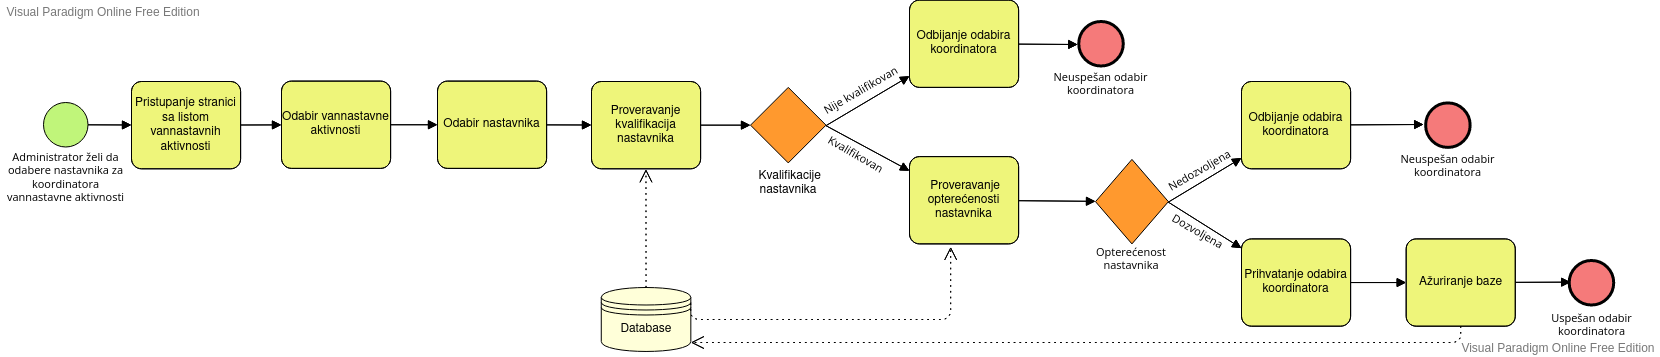
\includegraphics[scale=0.4]{imgs/BPMN_odabir_koordinatora.png}
    \end{center}
\caption{BPMN dijagram procesa Odabir nastavnika za koordinatora vannastavne aktivnosti}
\end{figure}
\end{landscape}

\section{Model baze podataka}

\begin{figure} [!ht]
    \begin{center}
        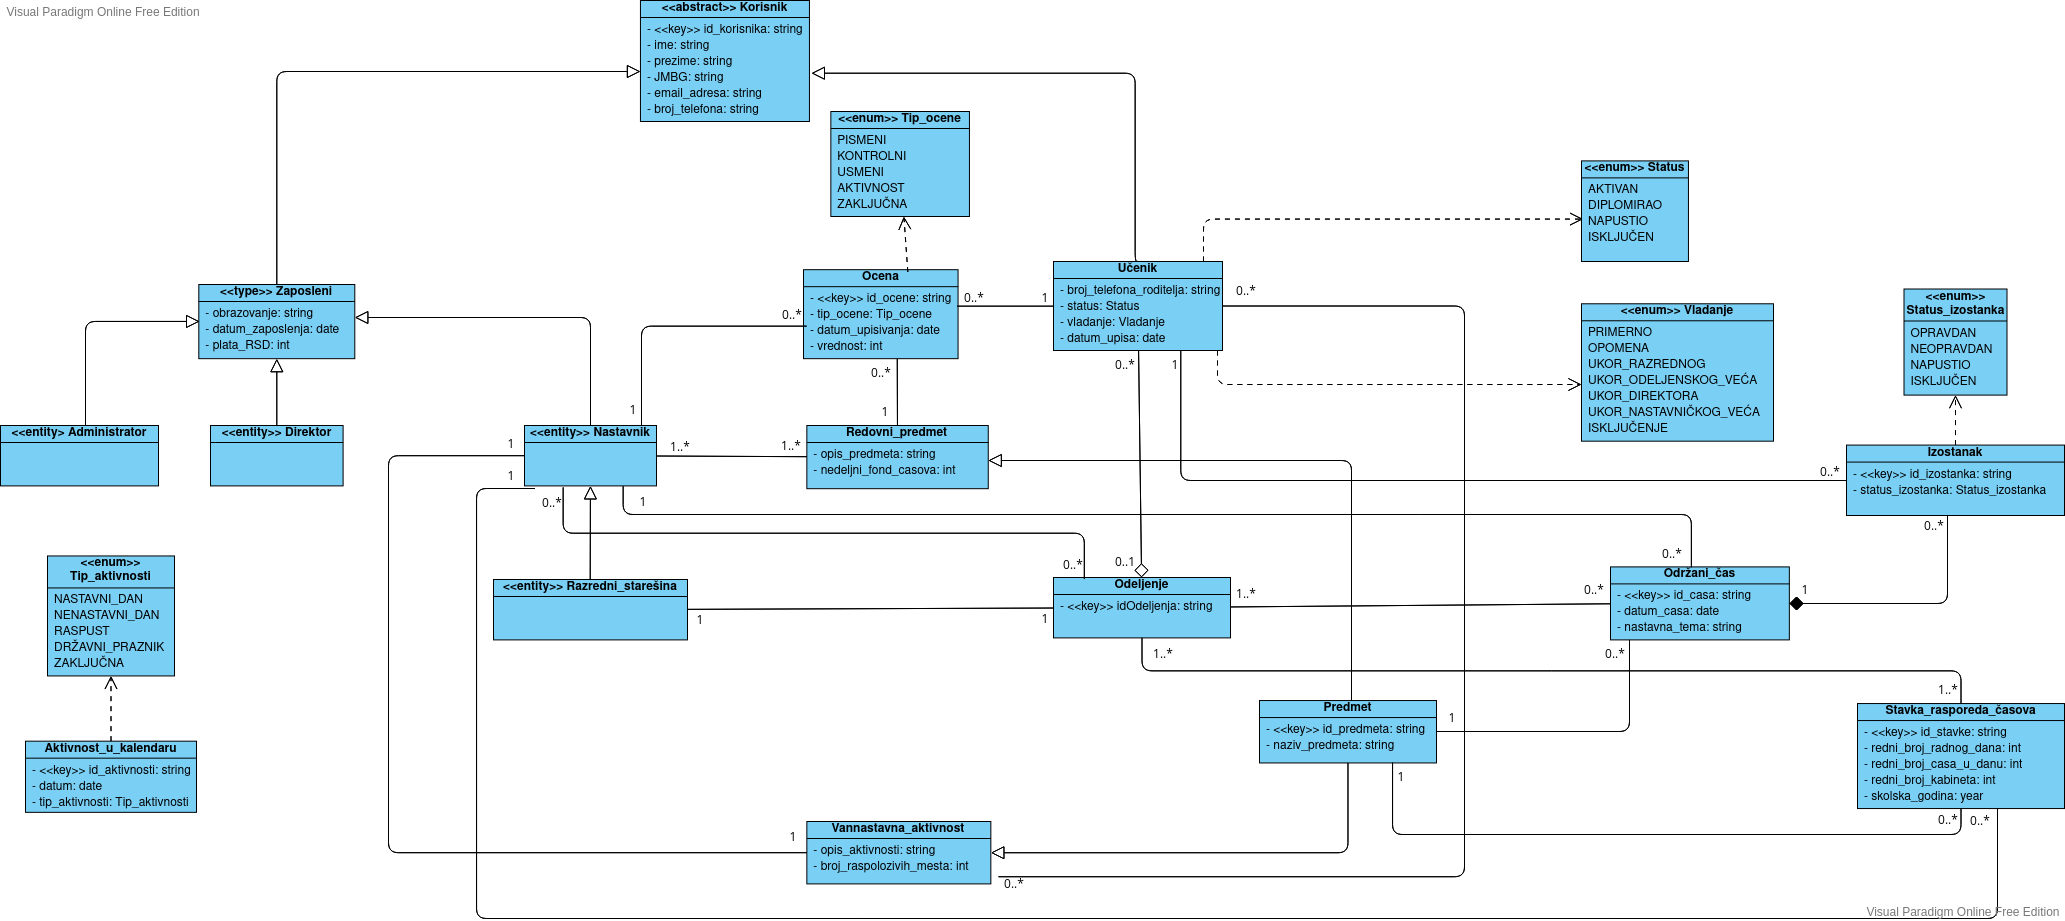
\includegraphics[angle=90,scale=0.22]{imgs/dijagram_klasa_podataka.png}
    \end{center}
\caption{Dijagram klasa podataka baze podataka}
\end{figure}


\section{Arhitektura sistema}

\subsection{Kratak opis arhitekture}

Pri razmatranju tipa arhitekture koji bi bio u skladu sa funkcionalnim i nefunkcionalnim zahtevima, koji su postavljeni pred sistem, izabrana je slojevita klijent-server arhitektura. Izdvojena su tri osnovna sloja:
\begin{enumerate}
    \item Prezentacioni sloj (korisnički interfejs) - Najviši sloj omogućava krajnjem korisniku interakciju sa aplikacijom (prikaz i unošenje podataka). Funkcionalnosti koje pruža specifične su za svaki tip korisnika. Pokreće se u Veb pregledaču. Tehnologije: HTML, CSS, JavaScript (React.js biblioteka).
    \item Logički (aplikativni) sloj - Predstavlja centralni deo poslovne logike aplikacije i služi kao posrednik u komunikaciji između dva krajnja sloja. Obrađuje informacije prikupljene na prezentacionom sloju. Dohvata, dodaje, briše ili menja podatke u sloju podataka. Tehnologije: Node.js, React.js.
    \item Sloj podataka - Obuhvata relacionu bazu podataka i sistem za upravljanje bazom podataka. Tehnologije: PostgreSQL
\end{enumerate}

Tip aplikacije je Veb aplikacija, podrazumeva jedan serverski i više klijentskih računara. Podela odgovornosti na tri sloja značajna je u kontekstu: bržeg razvoja aplikacije, povećane skalabilnost i pouzdanosti. Zbog namene aplikacije veoma je značajan aspekt sigurnosti - prezentacioni sloj i sloj podataka ne mogu komunicirati direktno, aplikativni sloj zadužen je da spreči potencijalne maliciozne napade (poput SQL Injection-a). Kao posledica prirode podataka veoma značajne su nam superiorne performanse koje PostgreSQL ima u odnosu na konkurenciju u slučaju rada sa velikim kolekcijama podataka i složenijim upitima (koji uključuju pisanje).

\newpage
\subsection{Dijagram arhitekture sistema}

\begin{figure} [!ht]
    \begin{center}
        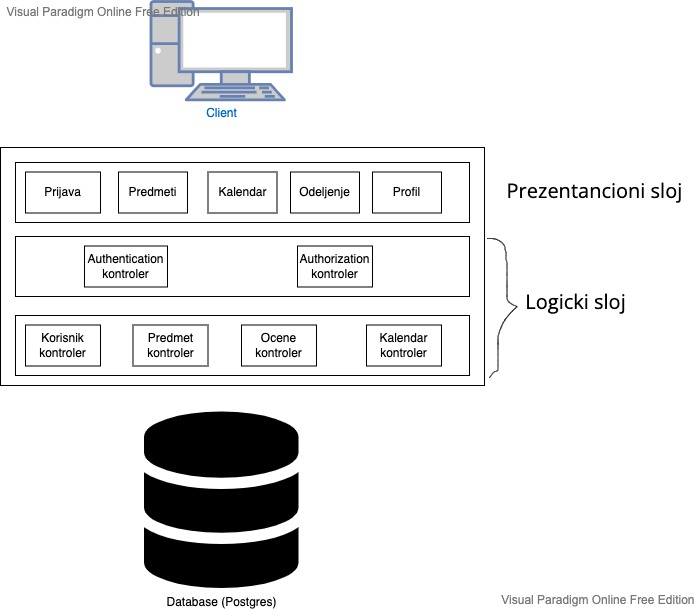
\includegraphics[scale=0.6]{imgs/arhitekturav2.jpeg}
    \end{center}
\caption{Dijagram arhitekture sistema}
\end{figure}

\newpage
\subsection{Dijagram komponenti sistema}
\begin{figure} [!ht]
    \begin{center}
        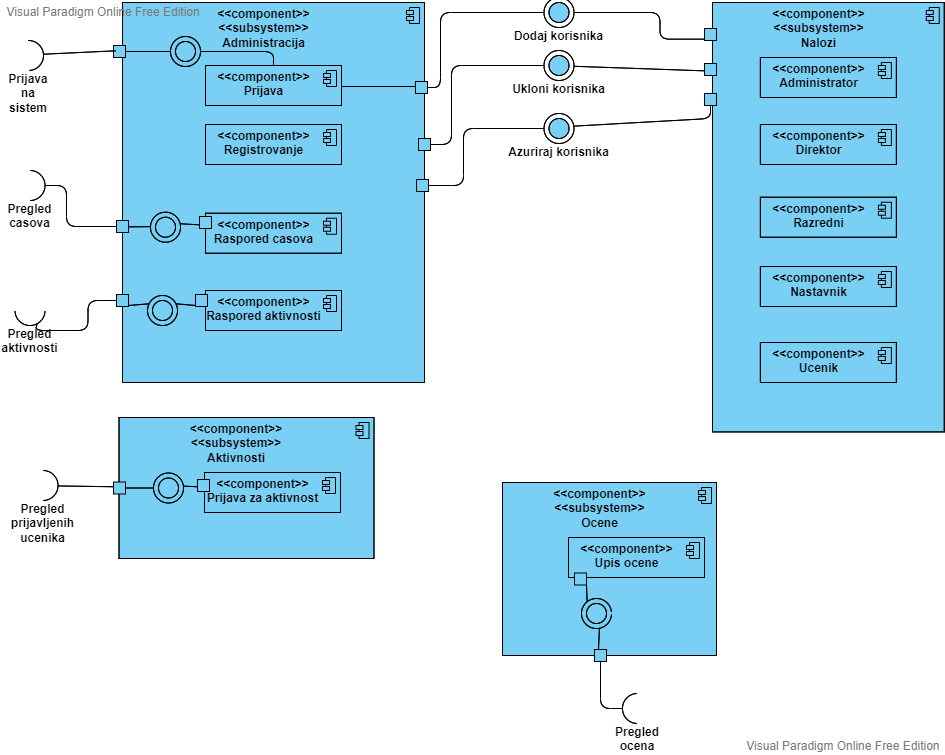
\includegraphics[scale=0.5]{imgs/dijagram_komponenti.png}
    \end{center}
\caption{Dijagram komponenti sistema}
\end{figure}

\newpage
\subsection{Dijagram isporučivanja sistema}
\begin{figure} [!ht]
    \begin{center}
        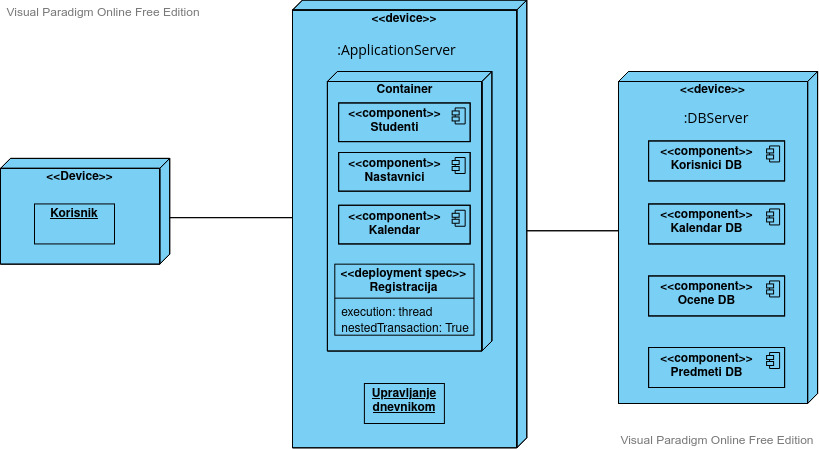
\includegraphics[scale=0.5]{imgs/Dijagram isporucivanja.vpd.jpg}
    \end{center}
\caption{Dijagram isporučivanja sistema}
\end{figure}


\end{document}
